\chapter{Calibration des jets avec les premi\`eres donn\'ees du run 1}
\label{chap:calibjets}

De tr\`es nombreux processus \'etudi\'es au LHC conduisent \`a la production de quarks et de gluons dans l'\'etat final de la collision. 
Une fois produits, les quarks et gluons s'hadronisent pour donner des jets collim\'es de particules sans couleur. 
Ces particules interagissent dans le d\'etecteur et les signaux produits, une fois regroup\'es en jets dits calorim\'etriques \`a l'aide d'un algorithme de reconstruction, constituent la signature exp\'erimentale des quarks et des gluons. 

La mesure des jets calorim\'etriques est fauss\'ee par plusieurs effets tels que la non-compensation des calorim\`etres, les pertes d'\'energies dans les parties non-instrument\'ees du d\'etecteur, les inefficacit\'es de reconstruction, etc.. 
%Ces effets doivent \^etre corrig\'es pour permettre une mesure pr\'ecise des processus physiques conduisant \`a la production de jets. 
L'ensemble des corrections appliqu\'ees pour corriger ces effets forment la calibration des jets. 
Avoir une calibration des jets pr\'ecise est crucial car elle est souvent une source d'incertitude importante lors de la mesure des processus physiques, comme 
par exemple lors des mesures des sections efficaces de production d'\'ev\'enements di-jets ou multijets~\cite{Aad:2014vwa,Aad:2013tea}, d'\'ev\'enements $t\bar{t}$~\cite{Aad:2014iaa} ou encore lors de la recherche de nouvelles r\'esonances se d\'esint\'egrant~en~jets~\cite{Aad:2014aqa}. 

%Les jets r\'esultants de l'hadronisation des quarks et gluons sont produits en grande quantit\'e dans les collisions de protons au LHC. Leur pr\'esence est exploit\'ee pour de nombreuses mesures et recherches de nouvelle physique. L'incertitude sur la mesure de l'\'energie des jets est, pour beaucoup d'entre elles, l'incertitude exp\'erimentale dominante. C'est le cas par exemple des mesures de section efficace de production d'\'ev\'enements di-jets ou multijets~\cite{Aad:2014vwa,Aad:2013tea}, d'\'ev\'enements top-antitop~\cite{Aad:2014iaa} ou encore de la recherche de nouvelles r\'esonances se d\'esint\'egrant en jets~\cite{Aad:2014aqa}. Avoir une mesure pr\'ecise de l'\'energie des jets est par cons\'equent d\'eterminant dans le programme de physique de l'exp\'erience \ATLAS. 

La stratégie d'\ATLAS~au début du run 1 était de mettre en place une calibration simple et robuste (nommée \EMJES) qui puisse être utilisée dans les analyses de physique rapidement et de développer en parallèle des calibrations plus sophistiquées qui pourraient, si elles s'avéraient performantes, être utilisées dans les analyses ultérieures. Une partie de mes travaux entre 2009 et 2012 a port\'e sur le d\'eveloppement d'une de ces m\'ethodes "sophistiqu\'ees" appel\'ee \english{Global Sequential}  (\GS) \english{Calibration}. Cette m\'ethode utilise les jets calibr\'es \`a l'\'echelle \EMJES~et leur applique des corrections suppl\'ementaires dans le but d'am\'eliorer leur r\'esolution en \'energie et de s'affranchir d'une partie de la d\'ependance avec la saveur. La reconstruction des jets et la calibration \EMJES~sont d\'ecrits succintement dans les sections \ref{sec:jetReco} et \ref{sec:EMJES}. La calibration \GS~est d\'ecrite dans la section \ref{sec:GS}. Ses performances et sa validation sur les donn\'ees sont d\'ecrites dans les sections~\ref{sec:performanceGS} et \ref{sec:systUncertGS}.

Les résultats pr\'esent\'es dans ce chapitre sur la calibration \GS{} sont le fruit d'un travail collectif r\'ealis\'e avec Reina Camacho, doctorante dans le groupe \ATLAS~du LPC entre 2009 et 2012 ayant travaill\'e sur cette calibration pendant la premi\`ere moiti\'e de sa th\`ese \cite{camacho:tel-00747143} et David Lopez Mateos et Ariel Schwartzman, initiateurs de cette calibration au sein d'\ATLAS. Ils sont pour la plupart tir\'es de la note~\cite{Busato:1365519} et de l'article~\cite{Aad:2011he}. Ce chapitre refl\`ete l'\'etat de la calibration des jets dans \ATLAS~\`a l'\'epoque o\`u cet article a \'et\'e \'ecrit et non celui au moment o\`u le pr\'esent document est publi\'e.

Dans ce qui suit, les résultats sur les données ont été obtenus sur le lot recueilli en 2010 à $\sqrt{s}=7~$TeV. La luminosité intégrée est de $38$~pb$^{-1}$. 

\section{Reconstruction des jets}
\label{sec:jetReco}

Les jets sont reconstruits par l'algorithme \antikt~\cite{Cacciari:2008gp} avec un param\`etre de distance $R=0,4$ ou $R=0,6$. Les objets utilis\'es en entr\'ee sont soit les amas dit "topologiques" reconstruits \`a partir des cellules des calorim\`etres \'electromagn\'etiques et hadroniques d'ATLAS~\cite{1748-0221-3-08-S08003}, soit les tours calorim\'etriques, soit les particules g\'en\'er\'ees dans le cas d'\'ev\'enements simul\'es. Dans ce qui suit, seuls les r\'esultats pour $R=0,6$ et pour les jets calorim\'etriques construits \`a partir des amas topologiques sont pr\'esent\'es. 

Les amas topologiques sont construits en regroupant les cellules voisines dont le rapport signal/bruit est grand. Leur utilisation permet de r\'eduire l'impact du bruit sur la reconstruction des jets et de l'\'energie transverse manquante et donc d'am\'eliorer les performances en terme d'identification et de r\'esolution. De plus, ils permettent une d\'efinition et une calibration des jets plus naturelle que celles obtenues avec les tours car ils sont l'image dans le calorim\`etre des gerbes \'electromagn\'etiques et hadroniques. %Le principe de l'algorithme de reconstruction des amas topologique est h\'erit\'e de l'algorithme "T42" de l'exp\'erience \Dzero \cite{D0noteUrsula, D0noteGregEmmJR, vlimantThesis, busatoThesis}, lui-m\^eme h\'erit\'e de l'exp\'erience H1. 

Apr\`es reconstruction, les jets calorim\'etriques sont \`a l'\'echelle dite \'electromagn\'etique (\EM). Cette \'echelle, d\'etermin\'ee par des tests en faisceaux, est telle que la r\'eponse est \'egale \`a 1 pour des \'electrons. 

Pour les \'ev\'enements simul\'es, les jets form\'es par les particules g\'en\'er\'ees sont reconstruits en utilisant le m\^eme algorithme que pour les jets calorim\'etriques. Toute les particules dont le temps de vie est sup\'erieur \`a 10~ps sont utilis\'ees \`a l'exception des muons et neutrinos. Ces jets servent de r\'ef\'erence dans les calibrations \EMJES~et \GS. Nous les appelerons par la suite les "jets de particules".

\section{Calibration \EMJES}
\label{sec:EMJES}

 La calibration \EMJES~corrige l'\'energie des jets calorim\'etriques de telle sorte \`a la ramener, en moyenne, \`a l'\'energie des jets de particules. Ceci a pour effet d'amener l'\'energie des jets \`a une \'echelle hadronique et donc de corriger 
%en partie 
la non-compensation des calorim\`etres \'electromagn\'etiques et hadroniques, les pertes d'énergies dans les parties non-instrumentées du détecteur, les inefficacités de reconstruction des amas topologiques, etc.. La direction des jets est \'egalement chang\'ee pour tenir compte de la position du vertex primaire et pour corriger du biais en $\eta$ provenant des d\'ep\^ots d'\'energie dans les r\'egions peu instrument\'ees du d\'etecteur. Cette calibration est d\'eriv\'ee sur un \'echantillon d'\'ev\'enements multi-jets simul\'es avec \pythia~(par la suite appel\'e \'echantillon nominal ou \'echantillon \pythia MC10) en fonction de la pseudorapidit\'e $\eta$ et de l'\'energie. Seuls les jets calorim\'etriques isol\'es associ\'es \`a un jet de particule isol\'e dans $\Delta R=3$ sont consid\'er\'es\footnote{$\Delta R=\sqrt{\Delta\eta^2+\Delta\phi^2}$}. Un jet est isol\'e si aucun autre jet d'impulsion transverse sup\'erieure \`a 7~GeV ne se trouve \`a moins de $\Delta R=2,5\times R$, o\`u $R$ est le param\`etre de distance de l'algorithme \antikt. 

La r\'eponse en \'energie
\[\langle\Response \rangle=\left<\frac{\Ecalo}{\Etruth}\right>\]
 \`a l'\'echelle \'electromagn\'etique est repr\'esent\'ee sur la figure \ref{fig:fig_09_responseEMscaleVsEta} en fonction de la pseudo-rapidit\'e pour diff\'erentes \'energies. Dans cette expression, $\Ecalo$ d\'esigne l'\'energie du jet calorim\'etrique, $\Etruth$ l'\'energie du jet de particule qui lui est associ\'e et $\left<\right>$ la moyenne sur les jets obtenue par un ajustement gaussien. Apr\`es calibration \EMJES, la r\'eponse est proche de 1. %Les facteurs correctifs \`a appliqu\'es pour atteindre un tel r\'esultat peuvent \^etre relativement grands. La figure \ref{fig:fig_09_responseEMscaleVsEta} montre que, \`a basse \'energie ils peuvent aller jusqu'\`a 2.

\begin{figure}[!h]
	\centering
	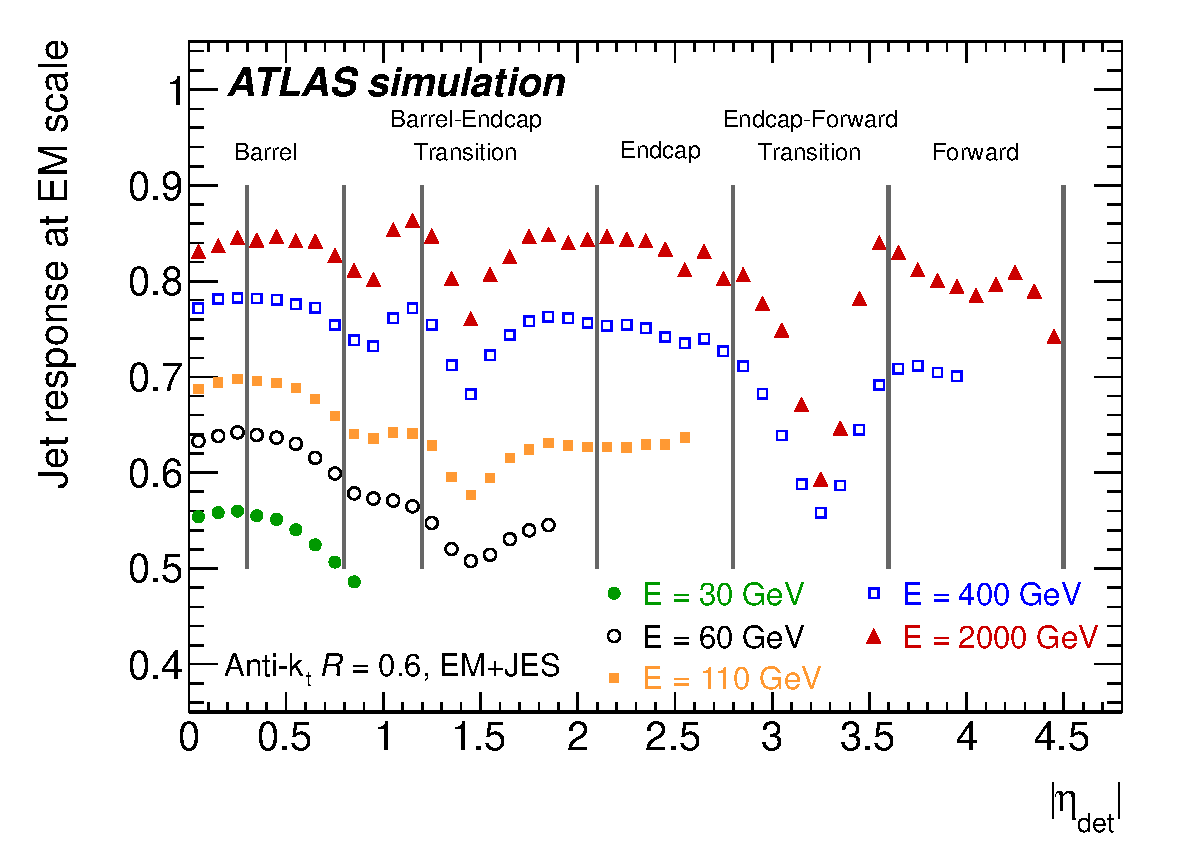
\includegraphics[scale=0.5]{figures/fig_09_responseEMscaleVsEta.pdf}
	\caption{R\'eponse en \'energie des jets \`a l'\'echelle \'electromagn\'etique en fonction de la pseudo-rapidit\'e pour diff\'erentes \'energies.}
	\label{fig:fig_09_responseEMscaleVsEta}
\end{figure}

L'incertitude sur l'\'echelle en \'energie \EMJES~provient de plusieurs sources :
\begin{maliste}
\item M\'ethode de calibration : cette incertitude est estim\'ee en appliquant la calibration sur l'\'echantillon utilis\'e pour la d\'eriver. 
\item R\'eponse en \'energie des calorim\`etres : cette incertitude est estim\'ee en propageant au jet l'incertitude sur la r\'eponse pour des hadrons isol\'es mesur\'ee soit \insitu~soit sur les donn\'ees du test en faisceau combin\'e de 2004.
\item Mod\'elisation du bruit dans les cellules calorim\'etriques : cette incertitude est estim\'ee en faisant varier le seuil sur le bruit dans la simulation
\item Mod\'elisation des mat\'eriaux dans le d\'etecteur : cette incertitude est estim\'ee en faiscant varier la quantit\'e de mat\'eriaux de diff\'erentes parties du d\'etecteur dans la simulation.
\item Mod\'elisation des \'ev\'enements dans les g\'en\'erateurs Monte Carlo : cette incertitude est estim\'ee en comparant la r\'eponse nominale (calcul\'ee sur l'\'echantillon \pythia~nominal) \`a la r\'eponse obtenue dans des \'echantillons simul\'es avec des mod\`eles de fragmentation, d'\'ev\'enement sous-jacent et de physique pour l'\'ev\'enement dur diff\'erent.
\end{maliste}

Les incertitudes associ\'ees \`a ces diff\'erentes sources ainsi que l'incertitude totale sont repr\'esent\'ees, pour la partie centrale du d\'etecteur, sur la figure \ref{fig:fig_22a_JES2010UncertaintyCentral}.

\begin{figure}[!h]
	\centering
	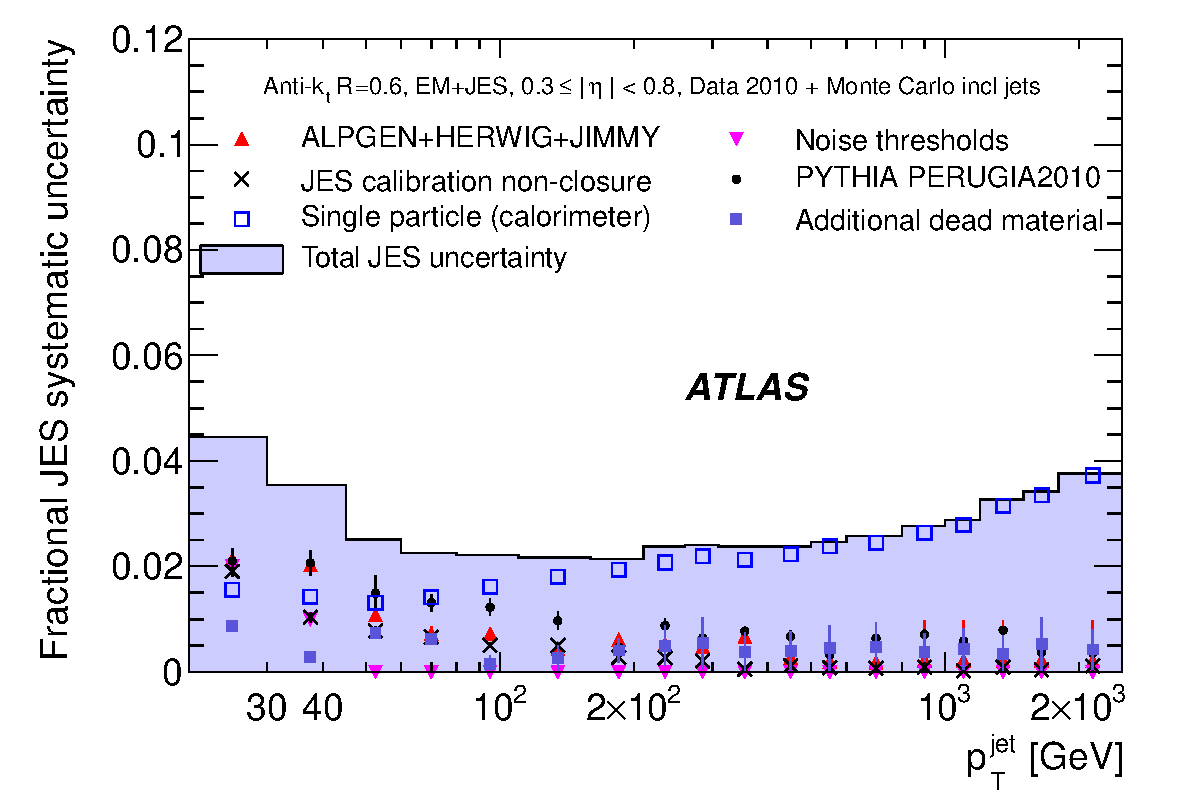
\includegraphics[scale=0.5]{figures/fig_22a_JES2010UncertaintyCentral.pdf}
	\caption{Incertitude syst\'ematique sur l'\'echelle en \'energie \EMJES~dans la partie centrale du d\'etecteur ($0,3\leq|\eta|<0,8$). Les contributions des diff\'erentes sources discut\'ees dans le texte sont montr\'ees, ainsi que l'incertitude totale (histogramme bleu).}
	\label{fig:fig_22a_JES2010UncertaintyCentral}
\end{figure}

\section{Calibration \GS}
\label{sec:GS}

La calibration \GS{} est une extension multivariée de la calibration EM+JES. Après la calibration EM+JES, la dépendance de la réponse avec $\eta$ et l'\'energie est supprimée. Cependant, la réponse peut dépendre d'autres variables comme celles caractérisant l'extension longitudinale et transversale des jets. La calibration \GS~supprime ces dépendances de manière séquentielle. Ses effets principaux sont d'am\'eliorer la résolution en énergie des jets et de réduire la dépendance de la réponse avec la saveur. 

Toute variable $x$ corr\'el\'ee avec la r\'eponse du calorim\`etre peut \^etre utilis\'ee. La r\'eponse en fonction de $x$ est d\'efinie par
\begin{equation} 
\label{eq:responsegsc}
                \langle \Response(x)  \rangle  =  \left<\frac{\ptjet(x)}{\pttrue}\right>
\end{equation}
o\`u \ptjet{} est l'impulsion transverse du jet calibr\'e \`a l'\'echelle \EMJES{} et \pttrue{} celle du jet de particule. Comme pour la calibration \EMJES{}, seuls les jets isol\'es associ\'es \`a un jet de particule isol\'e sont utilis\'es. La moyenne dans l'\'equation \ref{eq:responsegsc} est obtenue par ajustement gaussien dans un intervalle en  \pttrue, $\eta$ et $x$.

La d\'ependance de la r\'eponse en $x$ est supprim\'ee en multipliant $\ptjet$ par
\begin{equation}
\label{eq:gsc}
                C(x) = 1/ \langle \Response(x) \rangle.
\end{equation}
 
Plusieurs variables peuvent \^etre utilis\'ees de mani\`ere s\'equentielle pour atteindre la r\'esolution optimale. Cette proc\'edure requiert que la correction pour la variable $x_{n}$ soit calcul\'ee sur les jets pour lesquels les corrections pour les variables pr\'ec\'edentes aient d\'ej\`a \'et\'e appliqu\'ees. L'impulsion transverse d'un jet après la calibration \GS~est
\begin{equation}
\label{eq:ptGSaftercalib}
\pt^\GS=\left(\prod\limits_{n=1}^{N}C_n(x_n)\right)\times \pt^\EMJES
\end{equation}
où $N$ est le nombre de variables utilisées. Lors de l'application de cette procédure séquentielle, il faut prêter attention à ce que la correction pour la variable $n$ ne soit pas dégradée par les corrections $k>n$. Il a \'et\'e v\'erifi\'e que la r\'eponse en fonction de chaque variable ne change pas jusqu'\`a la derni\`ere correction. 

\subsection{Propri\'et\'es longitudinales et transversales des jets}

Les variables utilis\'ees dans la calibration \GS~(les $x_n$ dans l'\'equation \ref{eq:ptGSaftercalib}), sont des propri\'et\'es caract\'erisant la topologie longitudinale et transversale des d\'epots d'\'energie dans le jet. 
Une grande quantit\'e d'\'energie d\'epos\'ee dans les couches du calorim\`etre proches du point d'interaction indique que la gerbe a commenc\'e \`a se d\'evelopper en amont du calorim\`etre, induisant une r\'eponse plus faible puisqu'une partie de l'\'energie n'est pas d\'etect\'ee. 
Une grande fraction d'\'energie d\'epos\'ee dans le calorim\`etre hadronique indique une grande fraction hadronique au sein du jet conduisant \`a une r\'eponse plus faible (du fait de la non-compensation des calorimètres d'\ATLAS). 
Dans la partie centrale du d\'etecteur, une grande \'energie d\'epos\'ee dans la derni\`ere couche du calorim\`etre \'electromagn\'etique et dans la premi\`ere couche du calorim\`etre hadronique peut indiquer qu'une certaine fraction de l'\'energie du jet a \'et\'e perdue dans la partie non-instrument\'ee entre les deux calorim\`etres. 
La r\'eponse calorim\`etrique et l'extension transversale des jets sont corr\'el\'ees \`a la quantit\'e d'\'energie qui est perdue entre les parties tonneau et bouchon des calorim\`etres.

Chaque propri\'et\'e utilis\'ee peut \^etre sensible \`a plusieurs effets. Aucune tentative n'est faite pour s\'eparer ces effets dans la calibration \GS. Ils sont corrig\'es de mani\`ere implicite par les diff\'erentes corrections qui apparaissent dans l'\'equation \ref{eq:ptGSaftercalib}.

La structure longitudinale d'un jet (c'est-\`a-dire la structure le long de son axe), est caract\'eris\'ee par la fraction d'\'energie d\'epos\'ee dans les diff\'erentes couches des calorim\`etres \'electromagn\'etique et hadronique avant qu'une quelconque calibration en \'energie soit appliqu\'ee :
\begin{equation}
f_{\rm layer} = \frac{E_\EM^{\rm layer}}{E_\EM^{\rm jet}},
\end{equation}
o\`u $E_\EM^{\rm jet}$ est l'\'energie du jet \`a l'\'echelle \'electromagn\'etique et $E_\EM^{\rm layer}$ l'\'energie d\'epos\'ee dans la couche calorim\'etrique d'int\'er\^et, calcul\'ee \'egalement \`a l'\'echelle \'electromagn\'etique.

La structure transversale d'un jet (c'est-\`a-dire la structure dans le plan perpendiculaire \`a son axe) est d\'efinie par la largeur
\begin{equation}
\width = \frac{\displaystyle \sum_{i} p^i_{\rm T} \; \Delta R_{i,{\rm jet}}} {\displaystyle \sum_{i} p^i_{\rm T}},
\label{eq:jetwidth}
\end{equation}
o\`u la somme porte sur les amas topologiques formant le jet\footnote{Dans le cas de jets reconstruits \`a partir des tours calorim\'etrique la somme porte sur les tours.}, $p^i_{\rm T}$ est l'impulsion transverse de l'amas $i$ et $\Delta R_{i,{\rm jet}}$ est la distance dans le plan $\left(\eta,\phi\right)$ entre l'amas $i$ et l'axe du jet.

\subsection{D\'erivation des coefficients de calibration}

Les coefficients de calibration sont d\'etermin\'es dans tous les intervalles en $\eta$ de taille $0,1$ entre $|\eta|=0$ et $|\eta|=4,5$. Dans chaque intervalle, les propri\'et\'es permettant la meilleure am\'elioration de la r\'esolution en \'energie sont choisies. L'ensemble des propri\'et\'es formant la calibration \GS~ainsi que l'ordre dans lequel les corrections sont appliqu\'ees sont r\'esum\'es dans la table~\ref{tab:properties}. Dans cette table, \ftile~est la fraction d'\'energie d\'epos\'ee dans la premi\`ere couche du calorim\`etre hadronique dans la partie centrale,  \fem~celle d\'epos\'ee dans la derni\`ere couche du calorim\`etre \'electromagn\'etique dans la partie centrale, \fpres~celle d\'epos\'ee dans le pr\'e-\'echantillonneur dans la partie centrale, \fhec~celle d\'epos\'ee dans la premi\`ere couche du calorim\`etre hadronique dans la partie bouchon et \ffcal~celle d\'epos\'ee dans la premi\`ere couche du calorim\`etre \`a l'avant. La variable \width~est la largeur donn\'ee par l'\'equation~\ref{eq:jetwidth}. 

\begin{table}[ht!]
  \centering
  \begin{tabular}{c|c|c|c|c}
    \hline    \hline
r\'egion en $|\eta|$ & Corr 1 & Corr 2 & Corr 3 & Corr 4 \\
	    \hline
	$|\eta| < 1.2$     & \ftile & \fem  & \fpres & \width \\
	\etaRange{1.2}{1.4}   & \ftile &       &        & \width \\
	\etaRange{1.4}{1.7}   & \ftile & \fhec &        & \width \\
	\etaRange{1.7}{3.0}   &        & \fhec &        & \width \\
	\etaRange{3.0}{3.2}   &        & \fem  &        & \width \\
	\etaRange{3.2}{3.4}   &        & \fem  &        &       \\
	\etaRange{3.4}{3.5}   &        & \fem  &        & \width \\
	\etaRange{3.5}{3.8}   & \ffcal &       &        & \width \\
	\etaRange{3.8}{4.5}   & \ffcal &       &        &       \\
    \hline    \hline
  \end{tabular}
  \caption{S\'equence des corrections appliqu\'ees dans la calibration \GS~dans chaque intervalle en $|\eta|$.}
  \label{tab:properties}
\end{table}

Dans la suite de ce chapitre, \GSL~fait r\'ef\'erence \`a la calibration obtenue en appliquant seulement les corrections bas\'ees sur les fractions d'\'energie d\'epos\'ees dans les diff\'erentes couches calorim\'etriques (c'est-\`a-dire sans la correction bas\'ee sur la largeur) et \GS~\`a la calibration compl\'ete (incluant la correction bas\'ee sur la largeur).

L'effet de la calibration \GS~est montr\'e sur la figure \ref{fig:GSapply} dans le cas de \fem~et de la largeur \width. Dans les deux cas, la r\'eponse est montr\'ee avant et apr\`es calibration. Avant calibration, la r\'eponse d\'ecro\^it avec \fem~et \width. Apr\`es calibration, la d\'ependance de la r\'eponse avec ces deux variables est r\'eduite \`a moins de 1\% et la r\'eponse moyenne reste inchang\'ee. Un comportement similaire est observ\'e pour les autres variables.

\begin{figure*}[!ht]
\centering
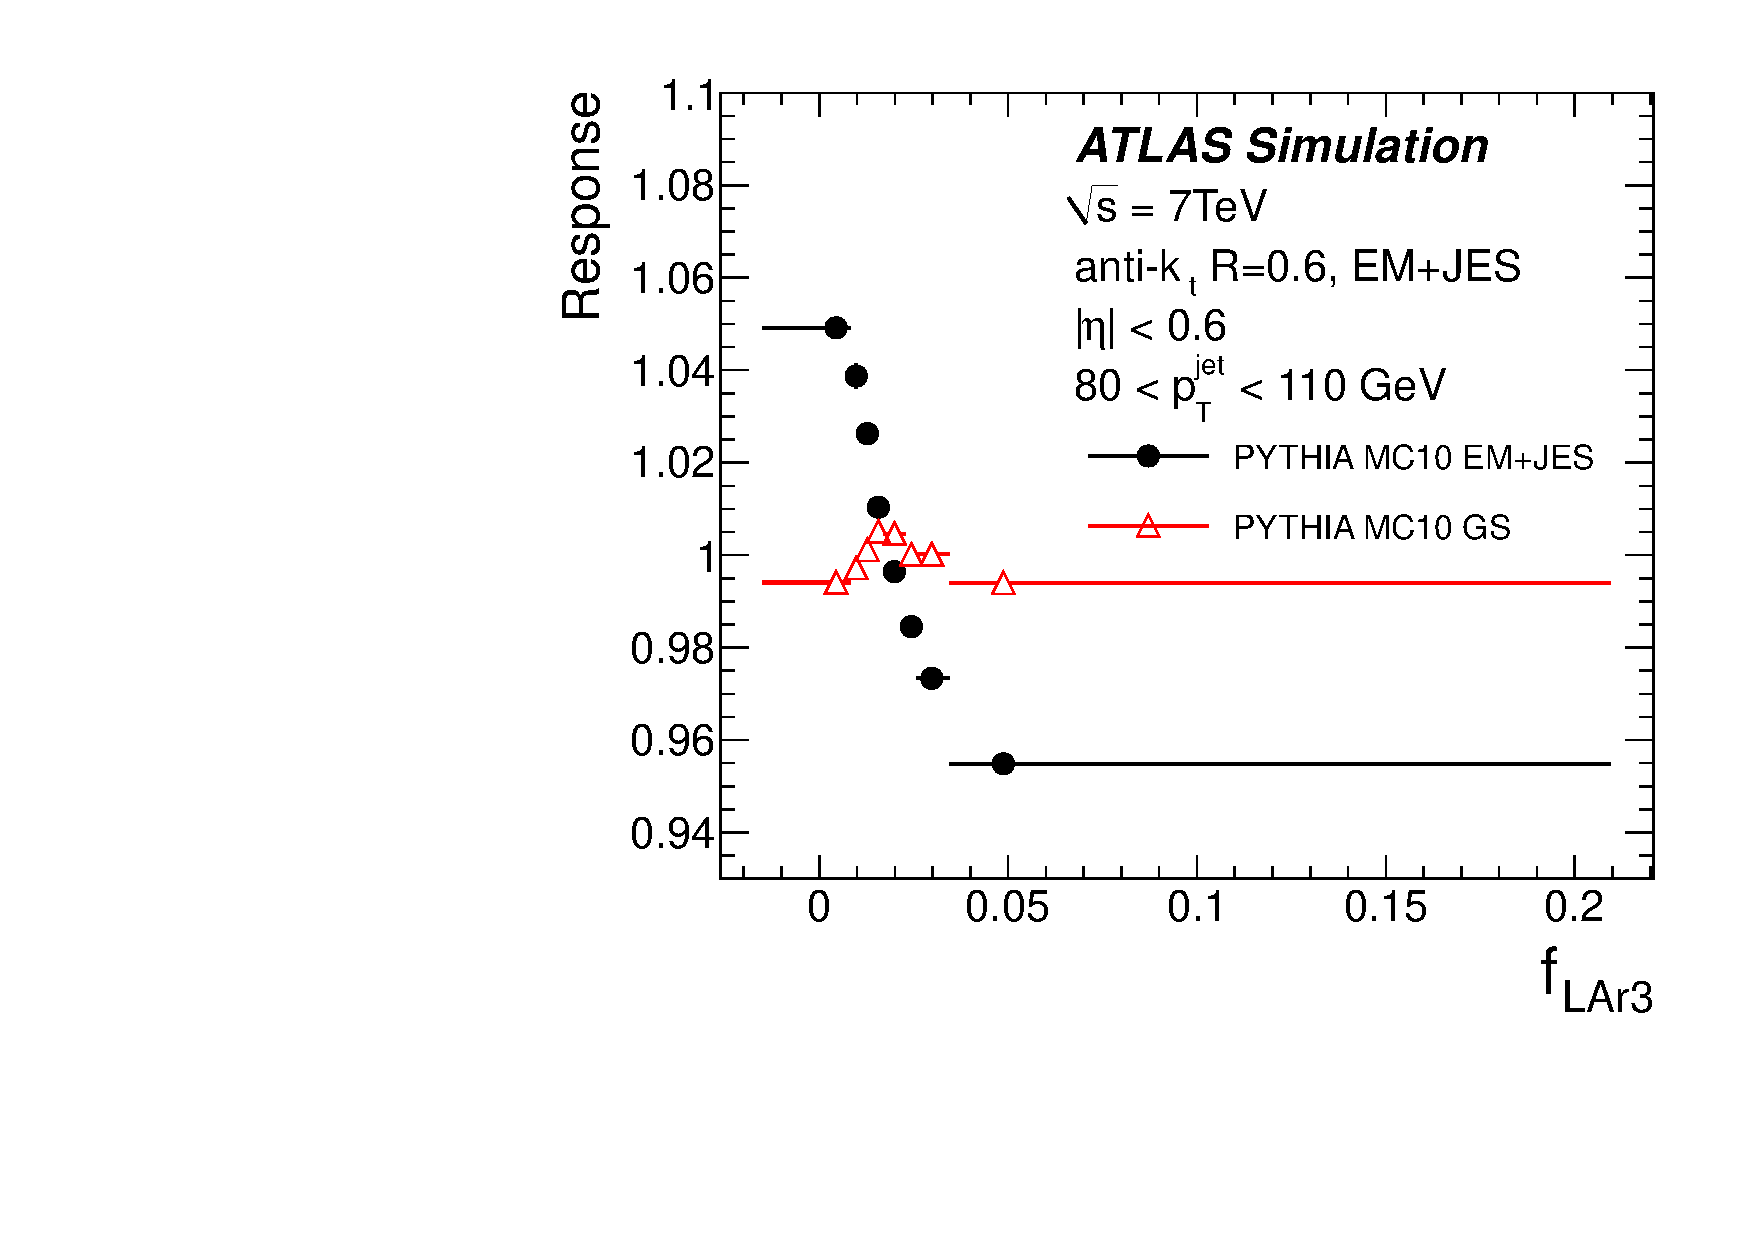
\includegraphics[width=0.44\textwidth]{figures/fig_46a.pdf}
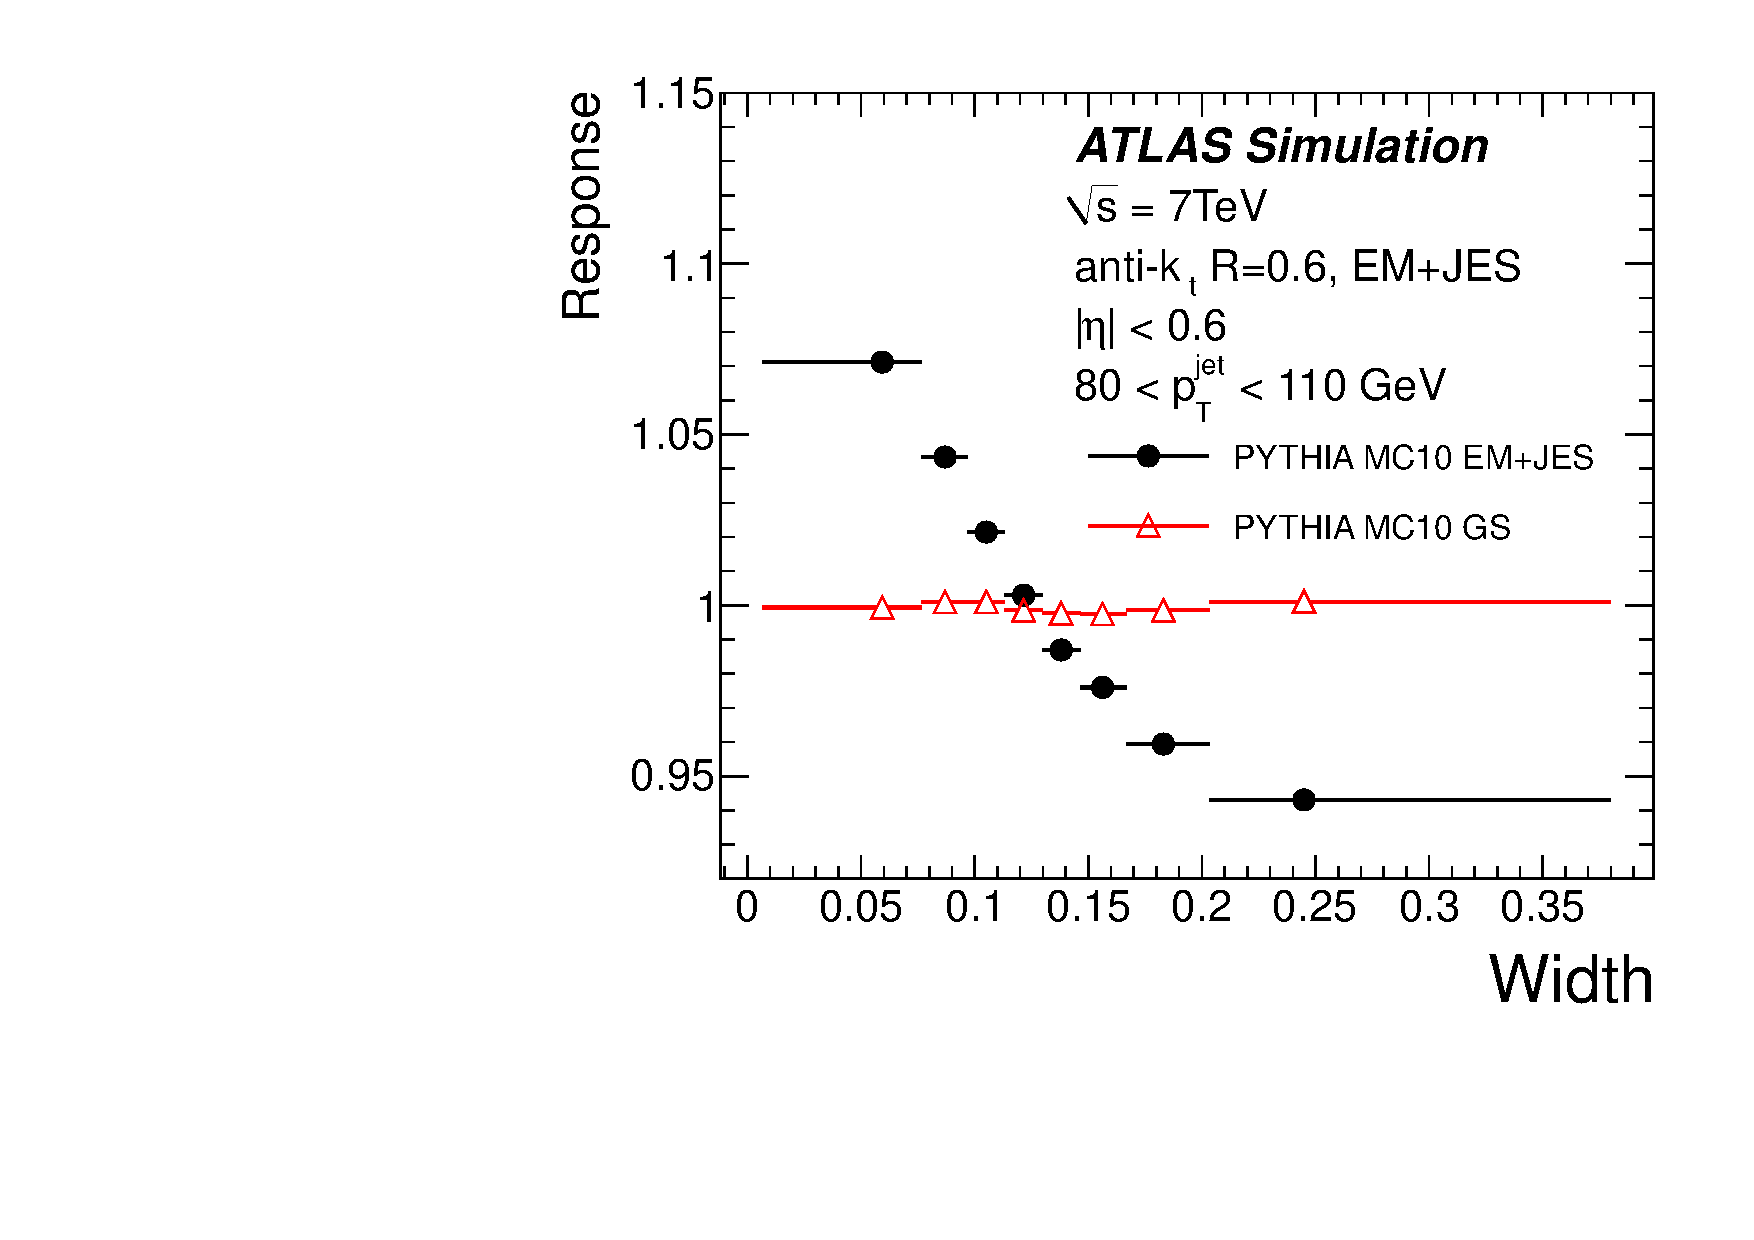
\includegraphics[width=0.44\textwidth]{figures/fig_46b.pdf}
\caption{R\'eponse en \'energie avant (ronds) et apr\`es (triangles) calibration \GS~en fonction de \fem{} (\`a gauche) et de la largeur du jet \width{} (\`a droite) pour les jets ayant $80 \le \pt < 110$~GeV et $|\eta|<0.6$.
}
\label{fig:GSapply}
\end{figure*}

\section{Performances de la calibration~\GS}
\label{sec:performanceGS}

De nombreuses études ont été réalisées afin de quantifier les performances de la calibration GS. %, aussi bien en terme de résolution en énergie que de dépendance en saveur. 
La r\'esolution en \'energie a été évaluée sur la simulation et sur les données. La figure~\ref{fig:fig_13a} montre la r\'esolution en \'energie sur les donn\'ees dans la partie centrale du calorim\`etre apr\`es les calibrations \EMJES~et \GS. Les r\'esultats pour les deux autres sch\'emas de calibration \'etudi\'es au d\'ebut du run~1, \LCW~et \GCW, sont \'egalement montr\'es (le lecteur int\'eress\'e par ces m\'ethodes peut consulter~\cite{Aad:2011he}). \GS{} permet d'améliorer la résolution de 20\% par rapport à EM+JES pour une impulsion transverse de 200~GeV dans la partie centrale ($|y|<0,8$, o\`u $y$ est la rapidit\'e). Pour $|y|\geq0,8$, l'am\'elioration est, pour cette impulsion transverse, de 20\%. Ces am\'eliorations sont comparables \`a celles obtenues avec les calibrations \GCW~et \LCW. 

\begin{figure}[!h]
	\centering
	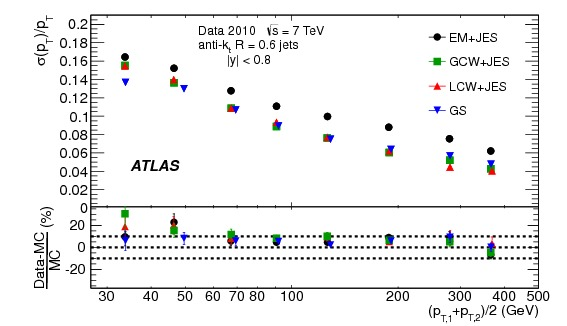
\includegraphics[scale=0.55]{figures/fig_13a.jpg}
	\caption{R\'esolution en \'energie en fonction de l'impulsion transverse pour les diff\'erents sch\'emas de calibration utilis\'es dans ATLAS. $p_{T,1}$ et $p_{T,2}$ sont les impulsions transverses des deux jets utilis\'es pour calculer la r\'esolution. La diff\'erence relative entre donn\'ees et simulation est montr\'ee sur la figure du bas.}
	\label{fig:fig_13a}
\end{figure}

Une attention importante a \'egalement \'et\'e donn\'ee \`a la quantification de la dépendance de la calibration en fonction de la saveur. En effet, les facteurs correctifs $C_n$ ont été déterminés sur un échantillon simulé multijets, enrichi en jets provenant de gluons. Ceux-ci sont toutefois appliqués à tous les jets, quelque soit leur provenance. Il est donc crucial de vérifier que les facteurs correctifs présentent une faible dépendance avec la saveur des jets. La réponse pour un échantillon pur de jets de gluons a \'et\'e comparée à celle pour un échantillon pur de jets de quarks dans la simulation. La figure~\ref{fig:fig_78a} montre la diff\'erence de r\'eponse entre les quarks l\'egers et les gluons dans la partie centrale du d\'etecteur. \GS~est la calibration qui pr\'esente la diff\'erence la plus faible. Les réponses diffèrent de 5\% à 20~GeV et de 0,5\% à 1 TeV. La calibration \GS~est \'egalement la calibration qui pr\'esente la plus faible diff\'erence dans la partie avant. Par exemple, dans la partie $2,1<|\eta|<2,8$, la diff\'erence est d'environ 1\% entre 30 et 400~GeV. Pour les autres calibrations, la diff\'erence est d'environ 5\% (3,5\%) pour \EMJES~(\LCW~et \GCW) \`a 30~GeV et d\'ecro\^it pour atteindre 1\% \`a 400~GeV.

%Deuxièmement, les facteurs correctifs issus de la simulation ont été appliqués sur des échantillons d'événements $\gamma$+jets réels et simulés, dans lesquels les jets sont majoritairement issus de quarks légers. Les différences observ\'ees sur ces \'ev\'enements sont du m\^eme ordre que celles observ\'ees sur la figure \ref{fig:fig_78a}.
%entre données réelles et la simulation n'excède pas 1\%, ce qui correspond à l'incertitude observée dans les échantillons enrichis en jets de gluons. 

\begin{figure}[!h]
	\centering
	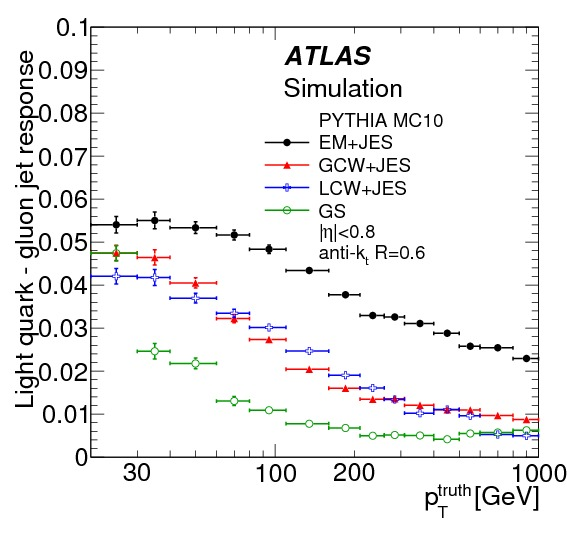
\includegraphics[scale=0.35]{figures/fig_78a.jpg}
	\caption{Diff\'erence entre la r\'eponse pour les jets issus de quarks l\'egers et la r\'eponse pour les jets issus de gluons pour les diff\'erents sch\'emas de calibration utilis\'es dans ATLAS.}
	\label{fig:fig_78a}
\end{figure}


\section{Incertitude sur l'\'echelle en \'energie apr\`es calibration~\GS}
\label{sec:systUncertGS}

Par construction, la calibration \GS~ne change pas l'\'energie moyenne des jets dans l'\'echantillon utilis\'e pour d\'eriver les facteurs correctifs $C_n$. Les imperfections de la simulation, une composition en saveur ou une topologie d'\'ev\'enements diff\'erents peuvent par contre conduire \`a des variations lorsque \GS~est appliqu\'e sur d'autres \'echantillons. La d\'ependance en saveur a d\'ej\`a \'et\'e discut\'ee dans la section~\ref{sec:performanceGS}. Dans cette section, les \'etudes r\'ealis\'ees afin d'\'evaluer l'incertitude syst\'ematique li\'ee aux autres effets sont pr\'esent\'ees.


\subsection{Validation de la calibration \GS~sur les donn\'ees}

Afin de v\'erifier que la calibration d\'eriv\'ee sur la simulation s'applique aux donn\'ees, les facteurs correctifs ont \'et\'e d\'eriv\'es directement \`a partir de ces derni\`eres puis compar\'es \`a ceux issus de la simulation. La m\'ethode utilis\'ee pour d\'eriver les facteurs sur les donn\'ees est d\'ecrite dans la section \ref{sec:DijetBalanceMethod}. La validation de cette m\'ethode sur la simulation est d\'ecrite dans la section \ref{sec:ValidationDiJetMC}. Finalement, la comparaison des facteurs correctifs obtenus sur les donn\'ees et simul\'ees est d\'ecrite dans la section \ref{sec:MCBased_vs_DataBased}.

\subsubsection{M\'ethode de d\'erivation des facteurs correctifs sur les donn\'ees}
\label{sec:DijetBalanceMethod}

Les facteurs correctifs peuvent \^etre d\'eriv\'es sur des \'ev\'enements di-jets en exploitant la balance en impulsion transverse. Les \'ev\'enements di-jets sont s\'electionn\'es en demandant que les deux jets de plus haut \pt~soient dos-\`a-dos ($\Delta \phi > 2.8$ radian) et dans la m\^eme r\'egion en pseudo-rapidit\'e. Le jet utilis\'e pour mesurer la d\'ependance de la r\'eponse avec la fraction d'\'energie ou la largeur est qualifi\'e de jet "sonde" (ou \english{probe} dans les \'equations ci-dessous) alors que l'autre jet est qualifi\'e de jet de r\'ef\'erence. Le choix du jet sonde et du jet de r\'ef\'erence \'etant arbitraire, les \'ev\'enements sont utilis\'es deux fois en inversant leurs r\^oles.

Les facteurs correctifs sont mesur\'es gr\^ace \`a l'asym\'etrie d\'efinie par 
\begin{equation}
\label{eq:AsymReco}
A(x) = \frac{\pt^{\rm probe}(x) - \pt^{\rm ref}}{\pt^{\rm avg}(x)},
\end{equation}
o\`u $x$ est une des propri\'et\'es utilis\'ees dans la calibration \GS~(voir table~\ref{tab:properties}) et $\pt^{\rm avg}$ est l'impulsion transverse moyenne des deux jets donn\'ee par 
\begin{equation}
\pt^{\rm avg} = (\pt^{\rm probe}+ \pt^{\rm ref})/2. 
\end{equation}

%Both $\pt^{\rm probe}$ and $\pt^{\rm ref}$ depend on $x$,  but in a given event the value of $x$ of the probe jet is different from that of the reference jet.  For this reason the dependence on $x$ is explicitly written in Equation~\ref{eq:AsymReco} only for the probe jet.

Les deux jets ont toujours des impulsions transverses d\'efinies \`a la m\^eme \'echelle. Ainsi, lorsque la $n^\text{i\`eme}$ correction est d\'etermin\'ee, les deux sont corrig\'es jusqu'\`a la correction $n-1$. La r\'eponse en fonction de $x$ est donn\'ee par :
\begin{equation}
 \langle \Response(x) \rangle = \left \langle \frac{\pt^{\rm probe}}{\pt^{\rm ref}} \right \rangle \simeq \frac{2 + \langle A(x) \rangle }{2 - \langle A(x) \rangle}. 
\label{eq:RespVsAsym}
\end{equation}

La mesure de la r\'eponse de cette mani\`ere suppose que l'asym\'etrie au niveau des jets de particules soit nulle. Ceci est vrai en moyenne mais pas dans un intervalle en $x$ donn\'e. L'asym\'etrie mesur\'ee $A(x)$ est par cons\'equent compos\'ee \`a la fois des effets li\'es au d\'etecteur (que nous cherchons \`a mesurer) et d'effets li\'es \`a la physique des jets sous-jacente. Afin de supprimer l'effet d'asym\'etrie au niveau des jets de particules, une nouvelle asym\'etrie est introduite :
\begin{equation}
\label{eq:Aprime}
A'(x) = A(x) - A_{\rm true}(x),
\end{equation}
o\`u $A(x)$ est donn\'e par l'\'equation~\ref{eq:AsymReco} et $A_{\rm true}(x)$ est donn\'e par :
\begin{equation}
\label{eq:Atruegsc}
A_{\rm true}(x) = \frac{p_{{\rm T},{\rm truth}}^{\rm probe}(x)-p_{{\rm T},{\rm truth}}^{\rm ref}}{p_{{\rm T},{\rm truth}}^{\rm avg}(x)},
\end{equation}
o\`u $p_{{\rm T},{\rm truth}}^{\rm avg}(x) = (p_{{\rm T},{\rm truth}}^{\rm probe}(x)+p_{{\rm T},{\rm truth}}^{\rm ref})/2$, $p_{{\rm T},{\rm truth}}^{\rm probe}(x)$ et $p_{{\rm T},{\rm truth}}^{\rm ref}$ sont les impulsions transverses du jet de particule sonde et du jet de particule de r\'ef\'erence respectivement. La variable $A_{\rm true}(x)$ est l'asym\'etrie au niveau des particules. La variable $x$ dans l'\'equation~\ref{eq:Aprime} est celle du jet calorim\'etrique associ\'e au jet de particule. Lorsque $A'(x)$ est utilis\'e \`a la place de $A(x)$ dans l'\'equation~\ref{eq:RespVsAsym}, l'effet d'asym\'etrie au niveau des jets de particules est supprim\'e et la r\'eponse ne d\'epend plus que des effets li\'es au d\'etecteur.

\subsubsection{Validation sur les \'ev\'enements simul\'es}
\label{sec:ValidationDiJetMC}

La m\'ethode d\'ecrite dans la section pr\'ec\'edente est valid\'ee sur la simulation en comparant les r\'eponses calcul\'ees par l'\'equation \ref{eq:RespVsAsym} aux r\'eponses calcul\'ees en utilisant les jets de particules (c'est-\`a-dire en les comparant aux r\'eponses utilis\'ees pour construire la calibration \GS~officielle). La figure~\ref{fig:DijetMethodMC} montre cette comparaison apr\`es la calibration \EMJES~pour $80 \le \ptjet < 110$~GeV et $|\eta| < 0,6$. Les r\'esultats obtenus sans et avec prise en compte de l'asym\'etrie au niveau des jets de particules sont montr\'es. L'effet de cette asym\'etrie est particuli\`erement important pour la fraction d'\'energie d\'epos\'ee dans le pr\'e-\'echantillonneur et la largeur. Il peut aller jusqu'\`a 4\% pour l'intervalle en \pt~consid\'er\'e sur la figure~\ref{fig:DijetMethodMC} et jusqu'\`a 8\% pour des impulsions transverses proches de 20~GeV. Ces effets sont r\'eduits \`a moins de 2\% lorsque la correction $A_{\rm true}$ est appliqu\'ee. 

\begin{figure*}[!ht]
\centering
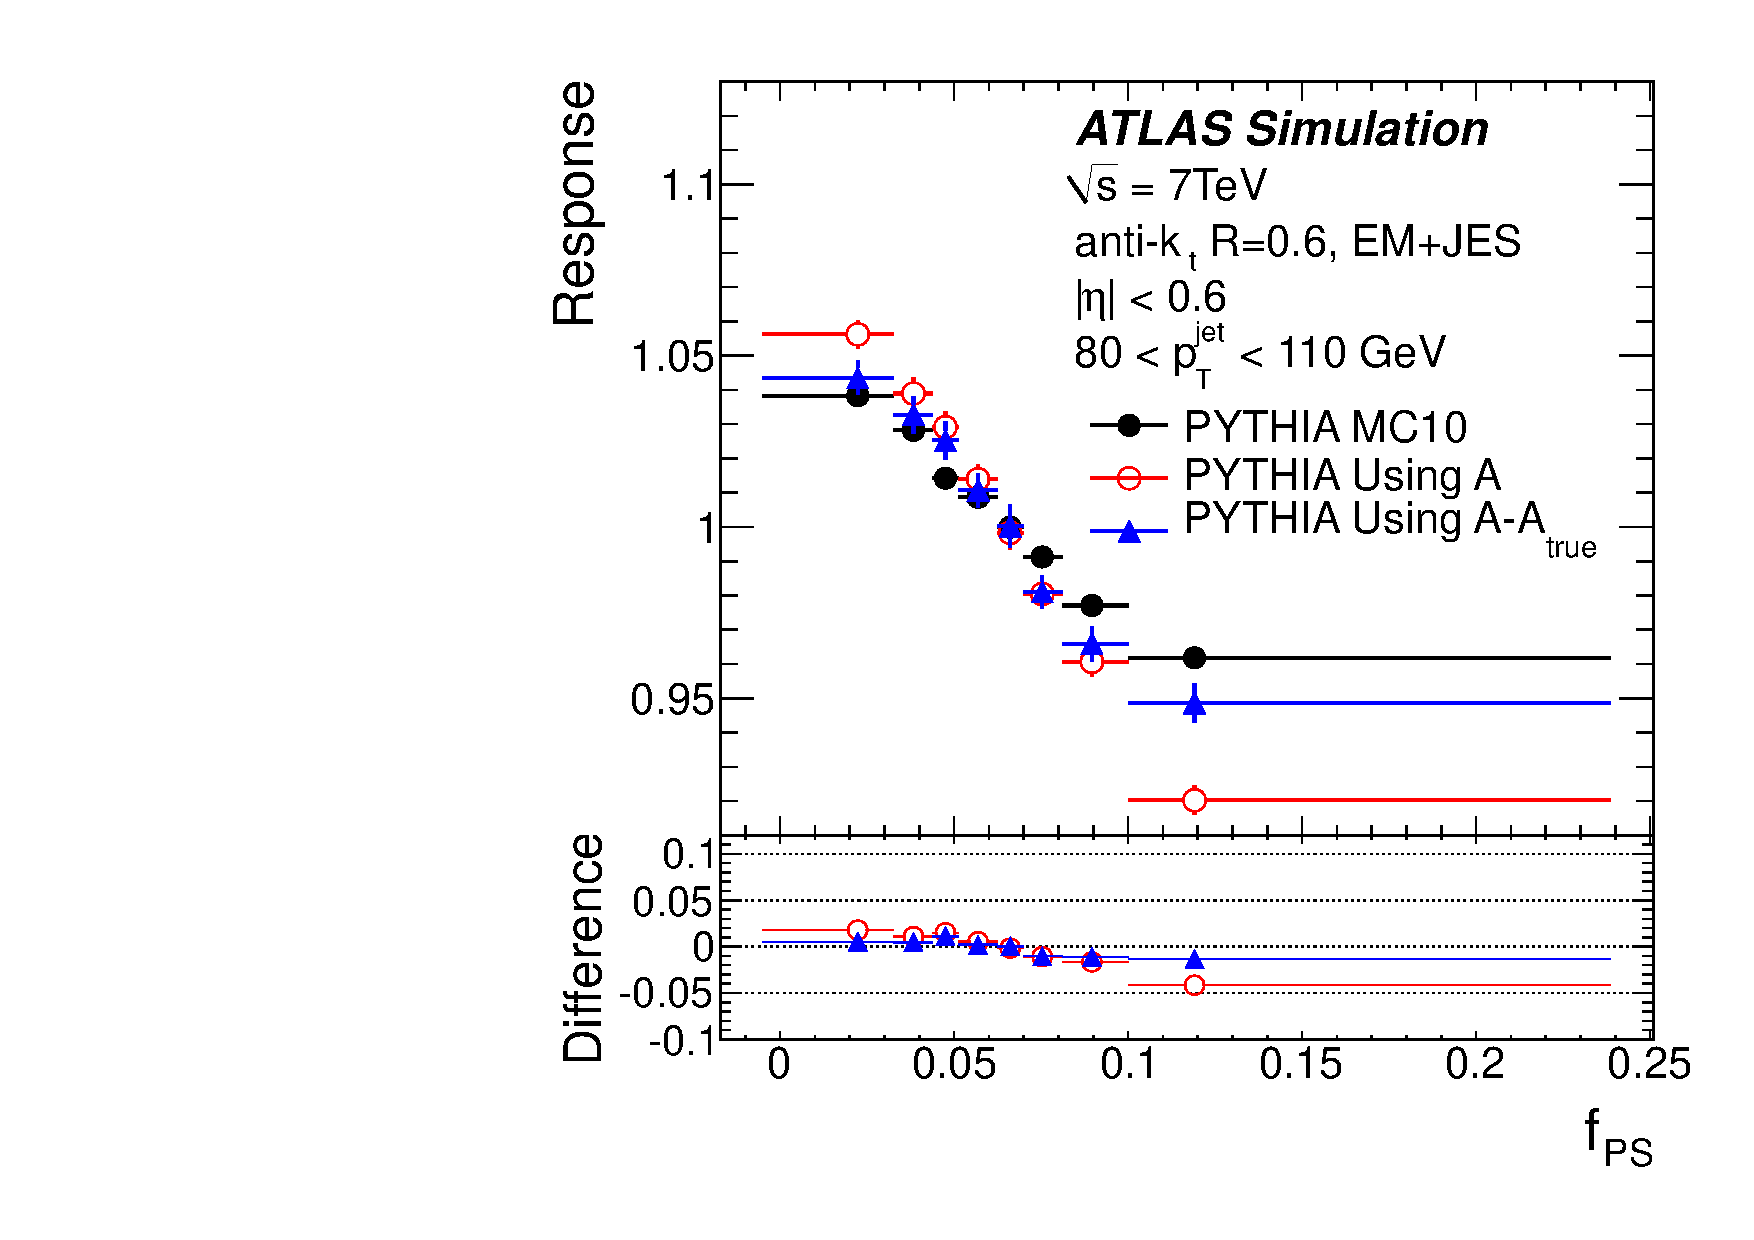
\includegraphics[width=0.4\textwidth]{figures/fig_47a.pdf}
\hspace{1.cm}
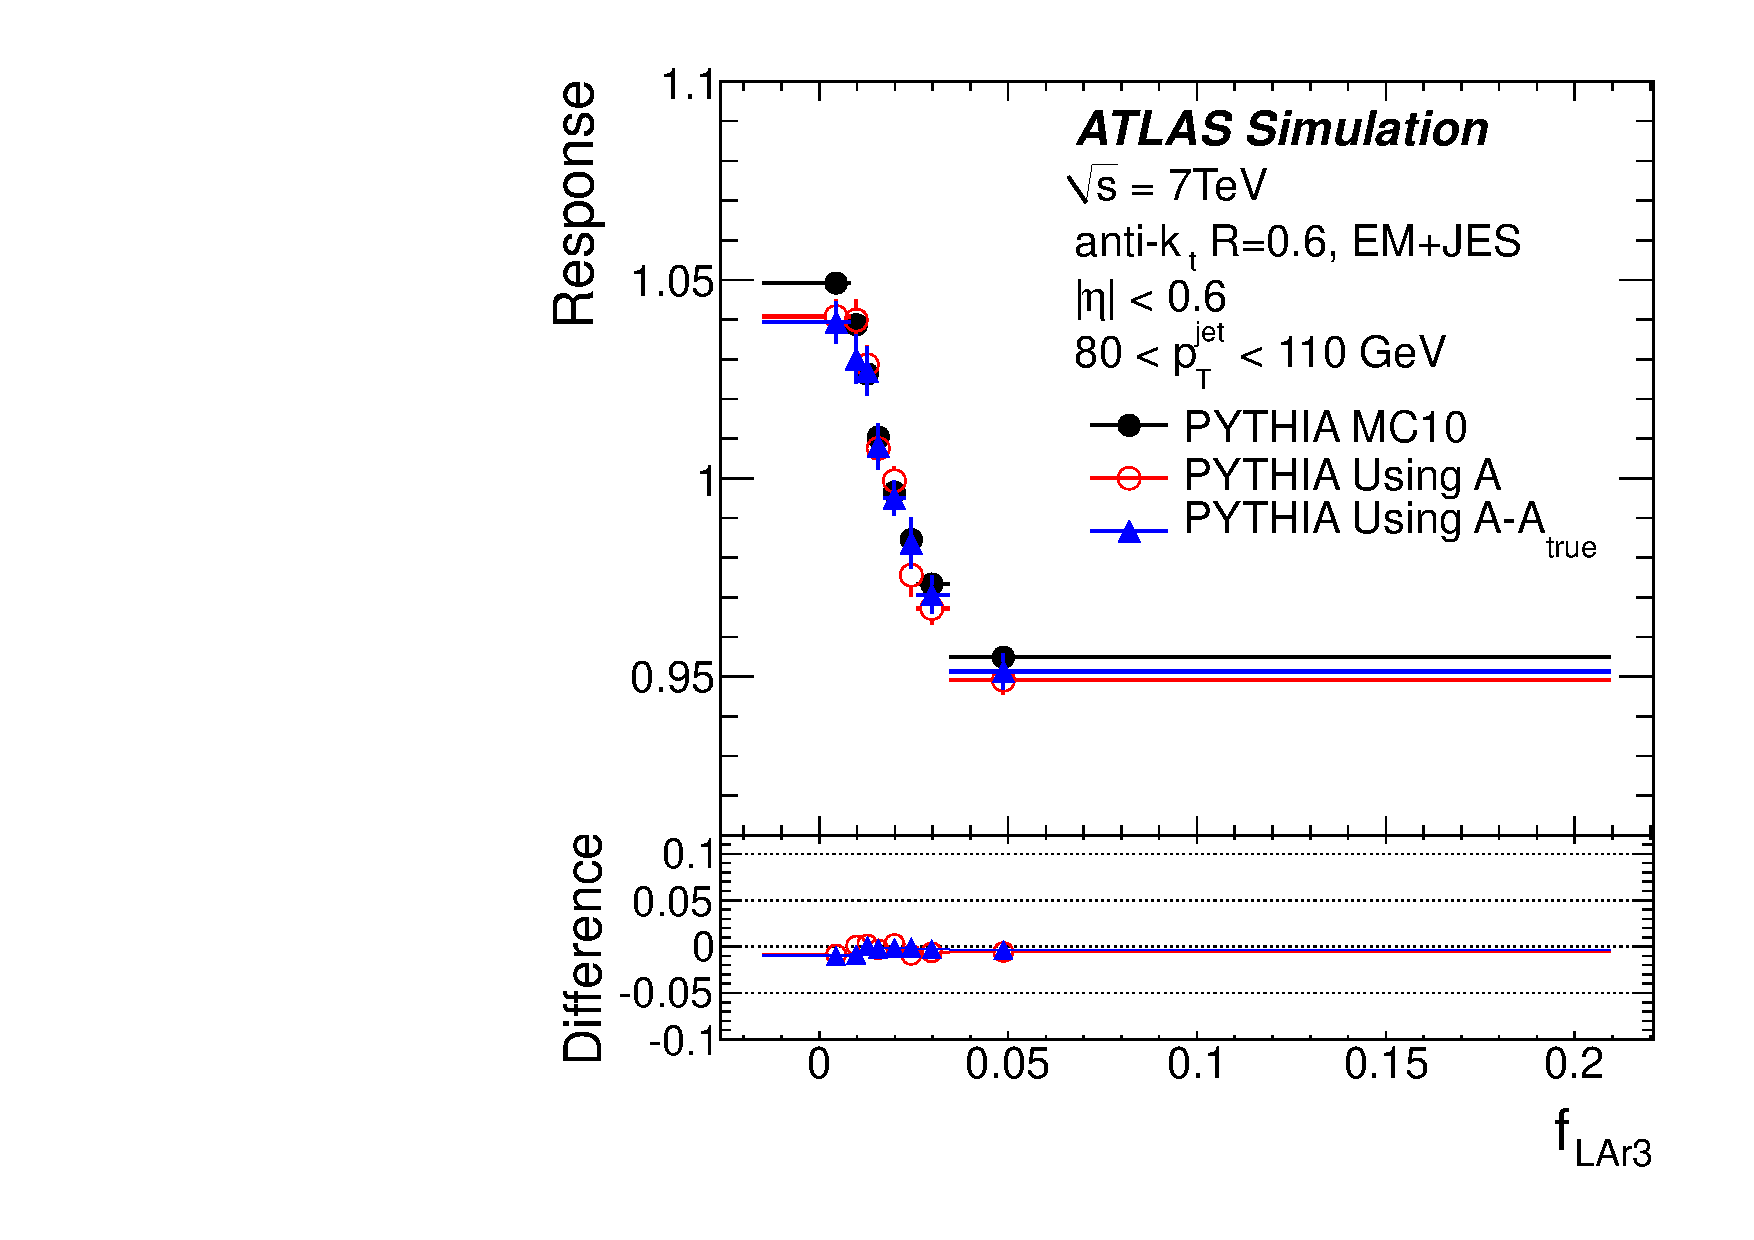
\includegraphics[width=0.4\textwidth]{figures/fig_47b.pdf}\\
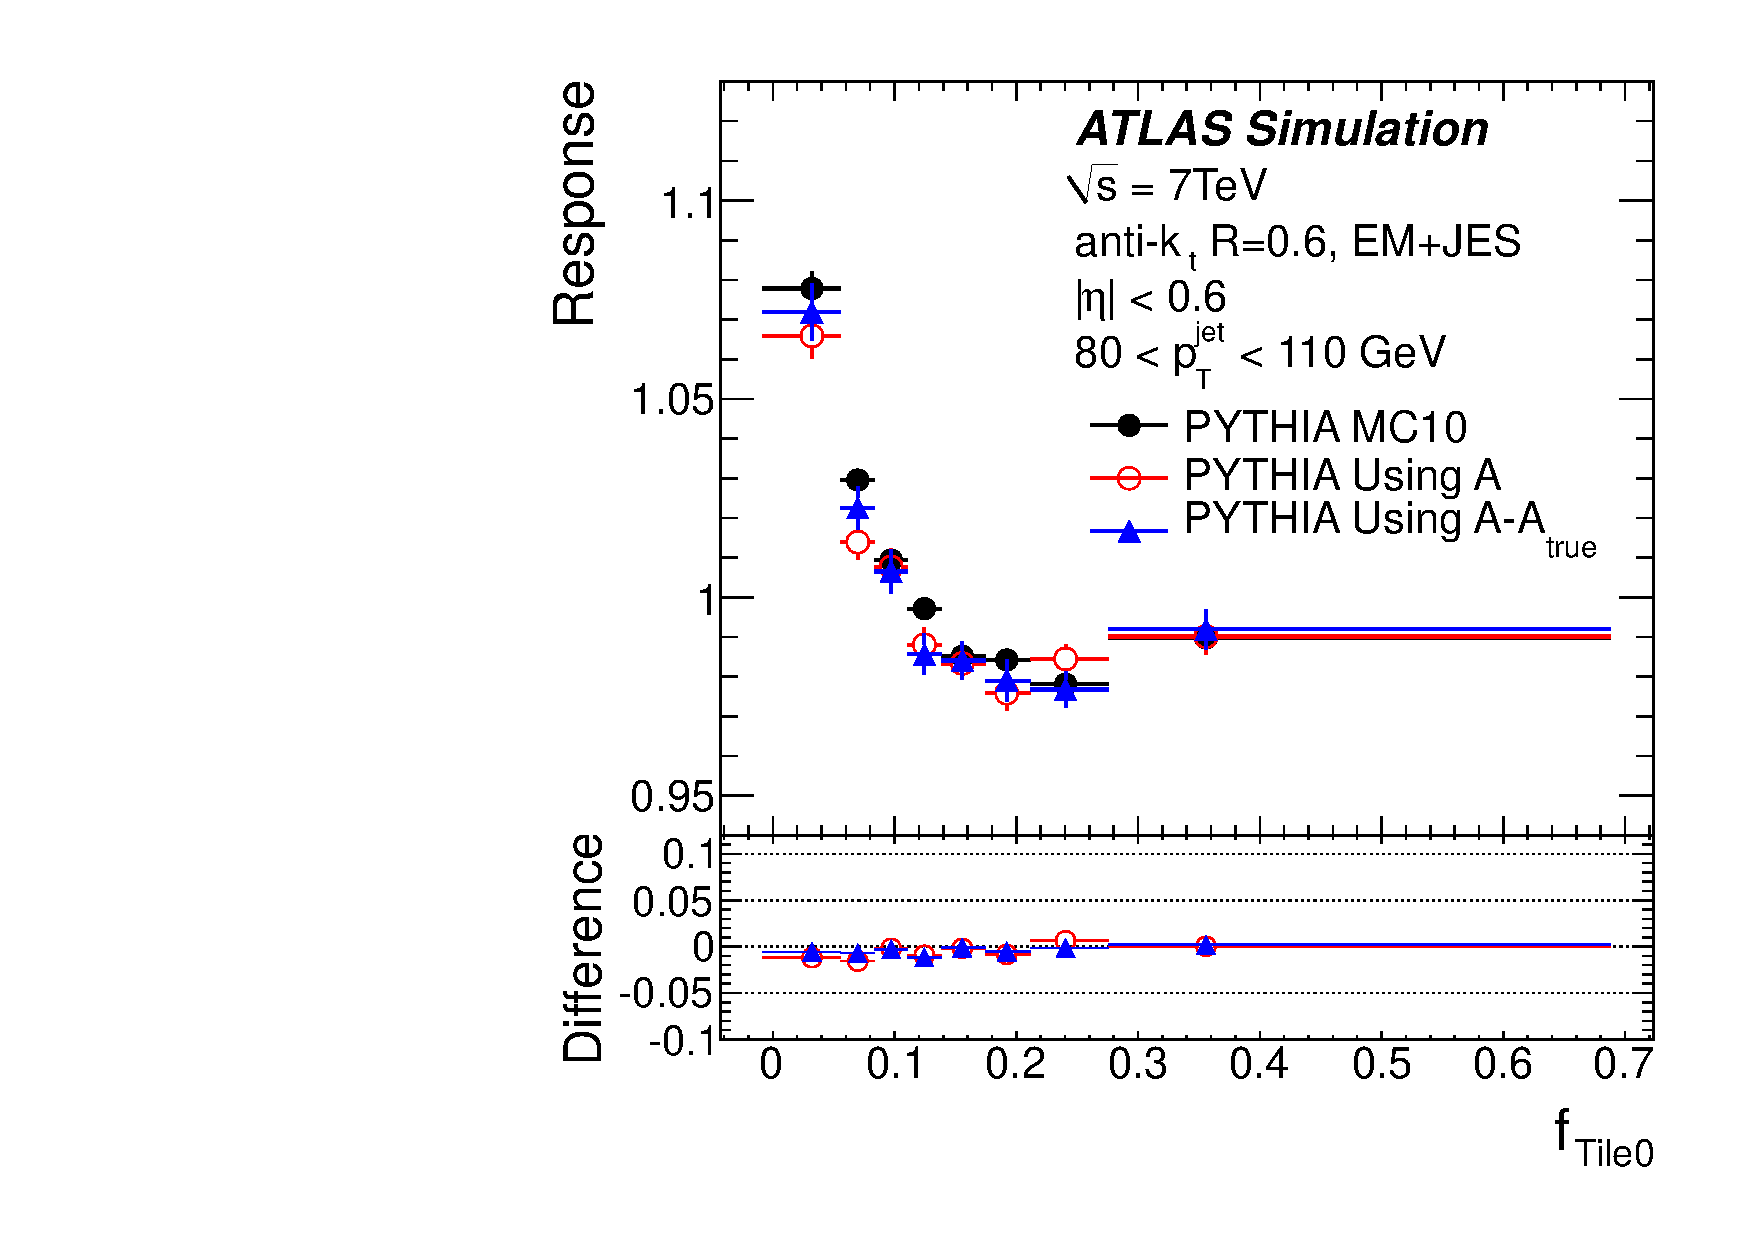
\includegraphics[width=0.4\textwidth]{figures/fig_47c.pdf}
\hspace{1.cm}
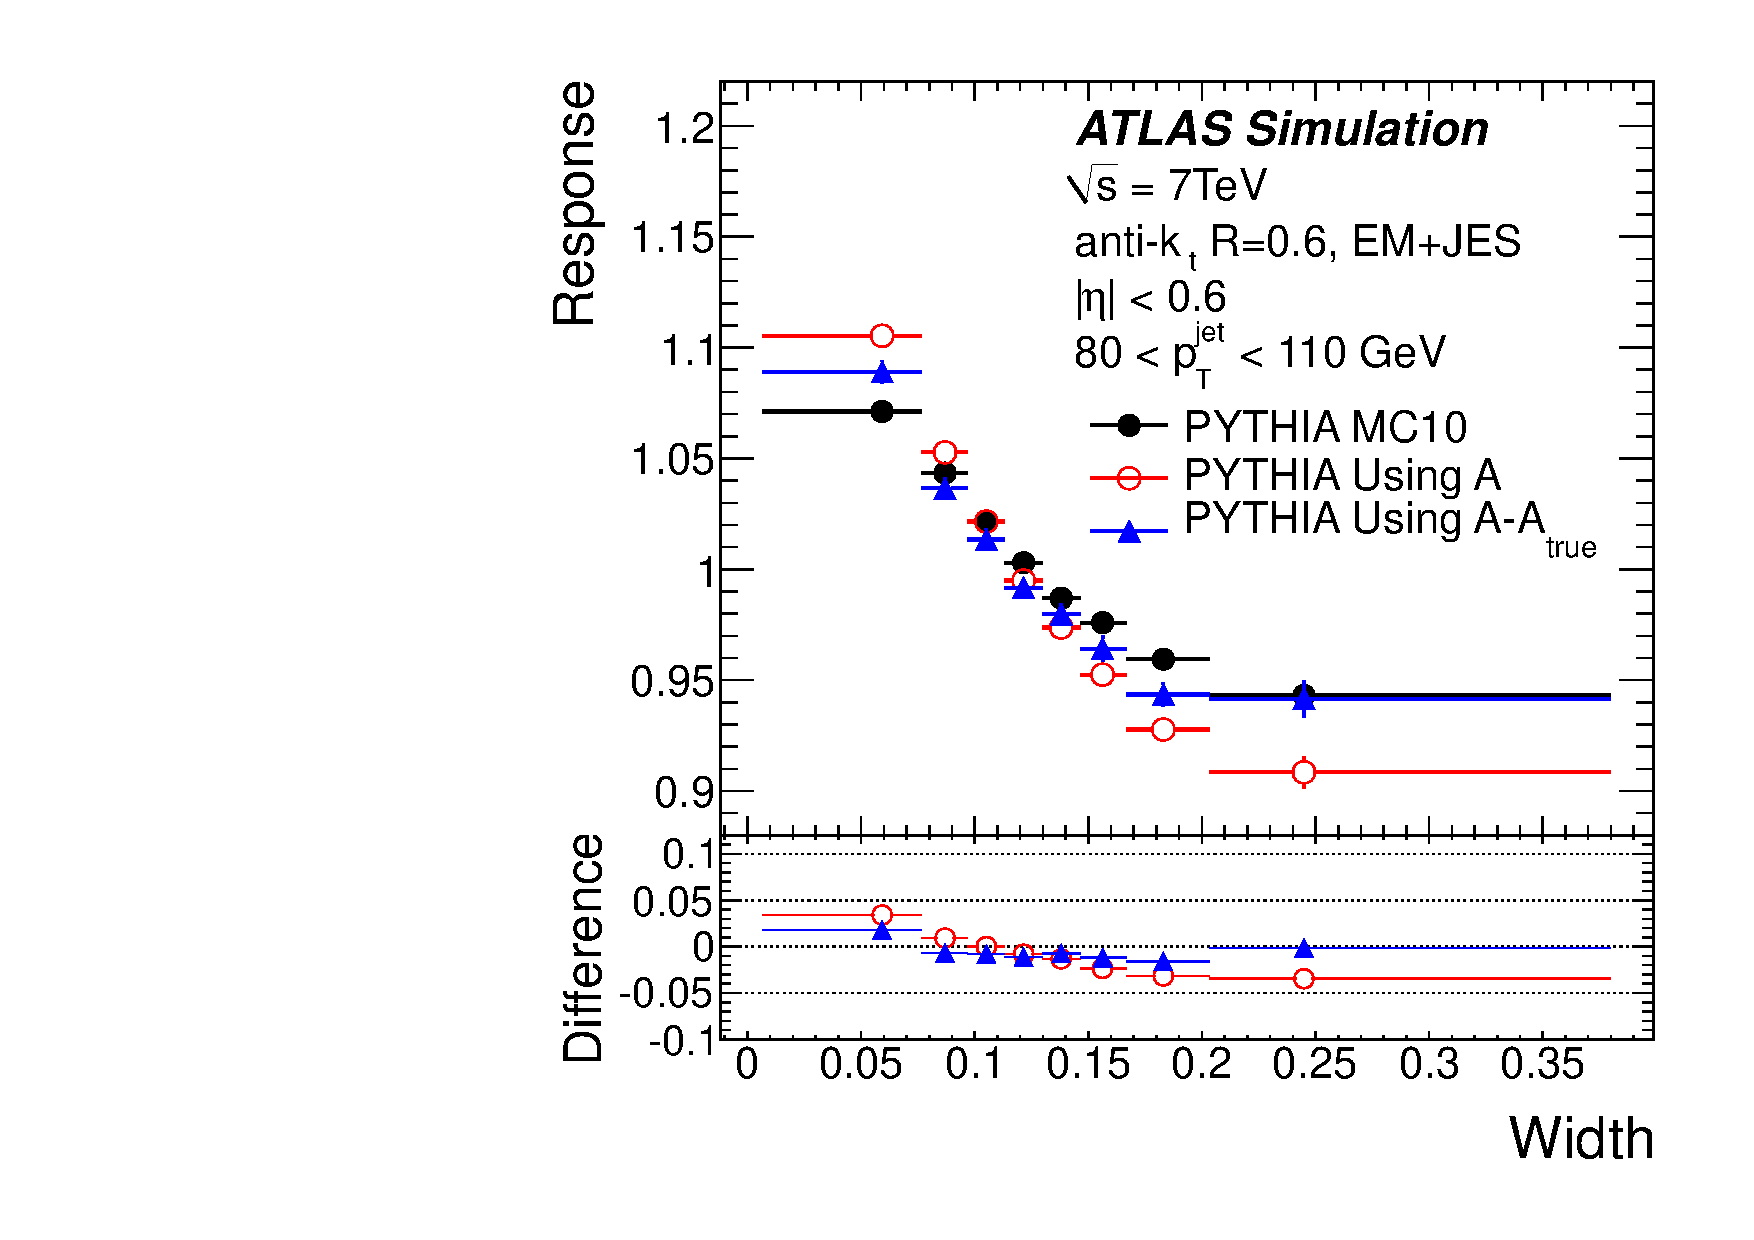
\includegraphics[width=0.4\textwidth]{figures/fig_47d.pdf}
\caption{R\'eponse en \'energie calcul\'ee avec les jets de particules (ronds pleins), l'asym\'etrie $A$ (ronds vides) et $A - A_{\rm true}$ (triangles) en fonction des fractions d'\'energie \fpres{}, \fem{}, \ftile{} et de la largeur \width~dans l'\'echantillon simul\'e nominal avant application de la calibration \GS. Les jets ont $80 \le \ptjet < 110$~GeV et $|\eta| < 0.6$. Pour chaque graphique, la diff\'erence entre la r\'eponse calcul\'ee avec les jets de particules et la r\'eponse calcul\'ee avec la m\'ethode bas\'ee sur l'asym\'etrie avec et sans prise en compte de $A_{\rm true}$ est montr\'ee.}
\label{fig:DijetMethodMC}
\end{figure*}

La robustesse de la correction bas\'ee sur $A_{\rm true}$ a \'et\'e test\'ee en mesurant cette asym\'etrie sur deux \'echantillons simul\'es en plus de l'\'echantillon nominal. Ces \'echantillons, appel\'es \Perugia2010 et \herwig++, diff\`erent de l'\'echantillon nominal par la mod\'elisation des radiations au niveau partonique, de l'hadronisation et des \'ev\'enements sous-jacents. La figure~\ref{fig:AtruthAllSamples} montre ces diff\'erentes mesures en fonction de \fpres{}, \fem{}, \ftile{} et de la largeur des jets dans la r\'egion centrale pour $40 \le \ptjet < 60$~GeV. L'asym\'etrie $A_{\rm true}$ ne diff\`ere pas de plus de $5 \%$ dans cet intervalle en \pt. Pour $\ptjet > 60$~GeV et les autres intervalles en $|\eta|$, les diff\'erences sont inf\'erieures \`a 2\%. \`A bas \ptjet{} (en dessous $40$~GeV dans la partie centrale), la coupure en $\Delta \phi$ combin\'ee avec la relative petite taille des \'echantillons \Perugia 2010 et \herwigpp{} conduit \`a des incertitudes statistiques de l'ordre de 5\%, ce qui emp\^eche de conclure de mani\`ere d\'efinitive sur un \'eventuel d\'esaccord.

\begin{figure*}[ht!]
\centering
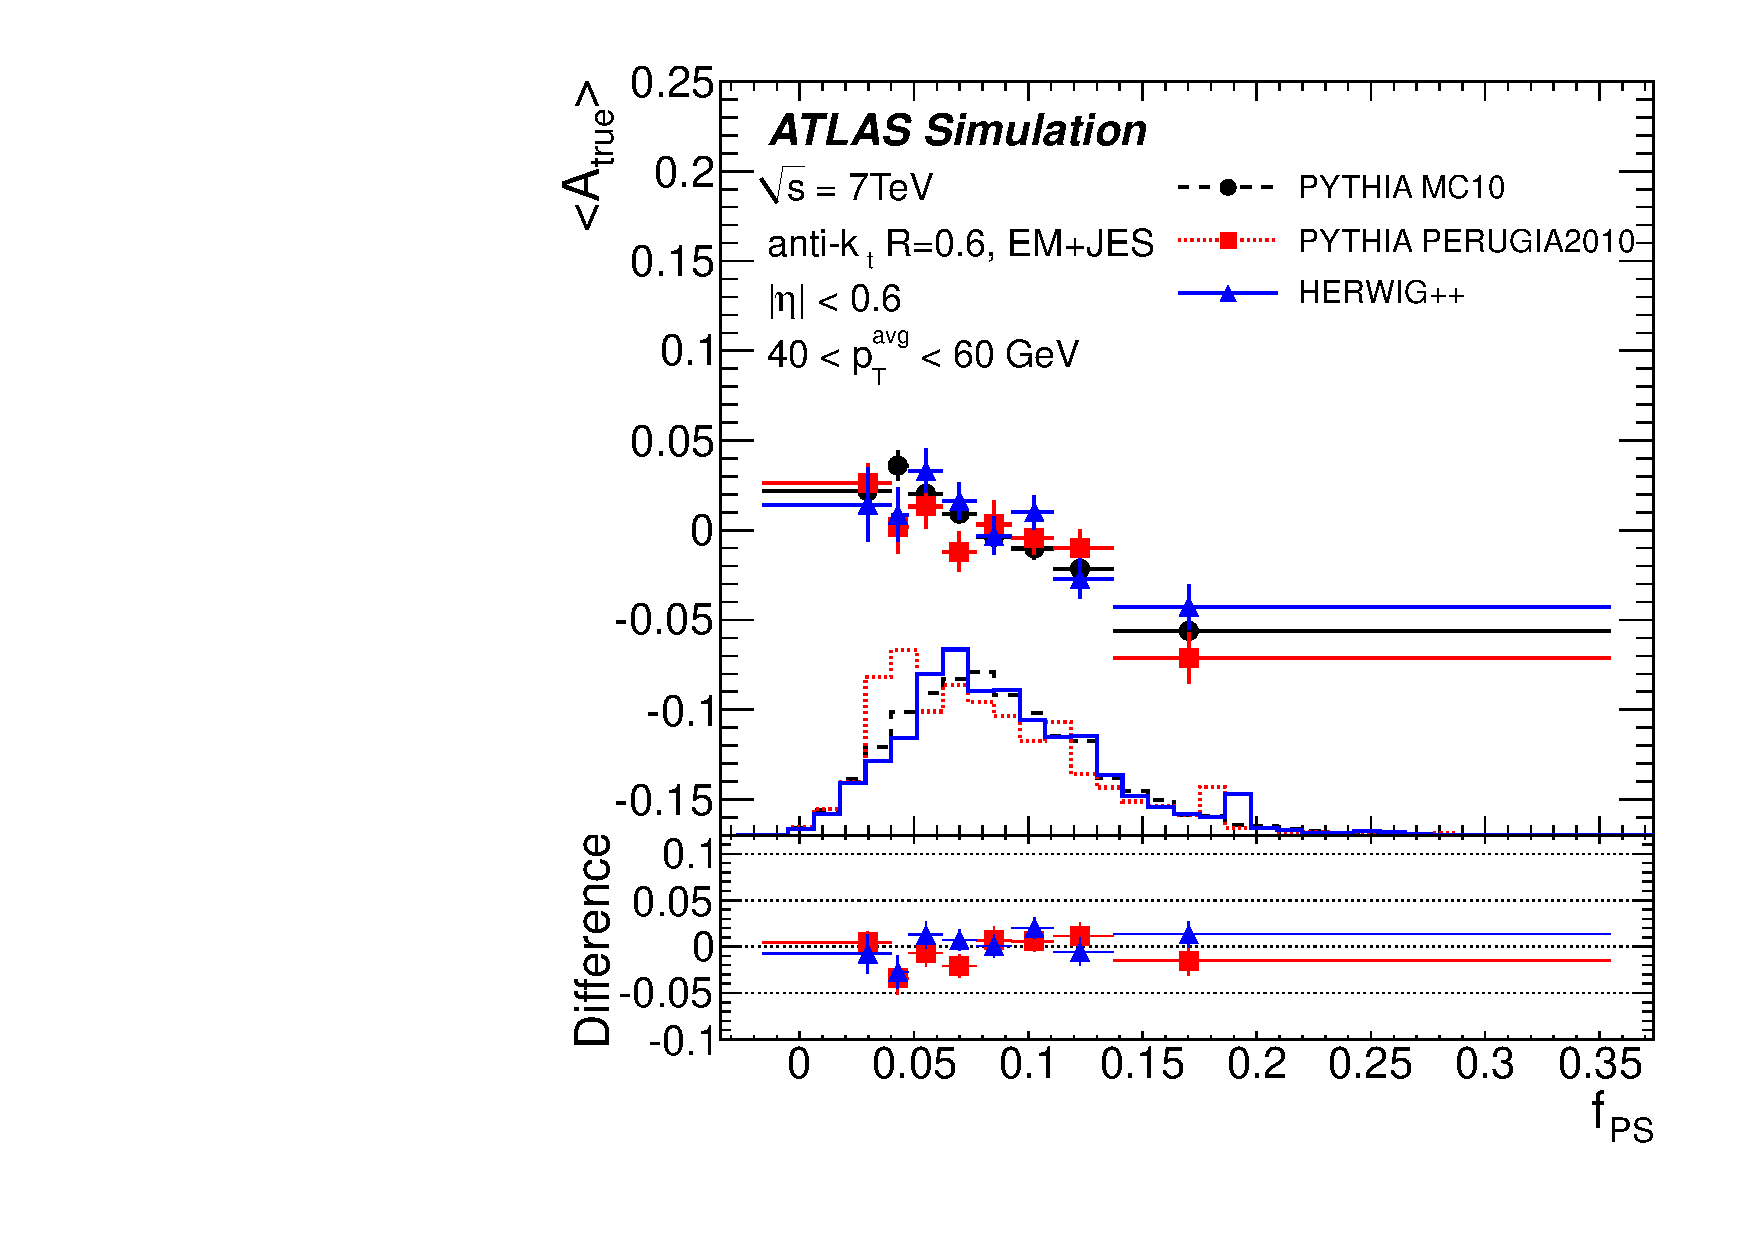
\includegraphics[width=0.4\textwidth]{figures/fig_48a.pdf}
\hspace{1.cm}
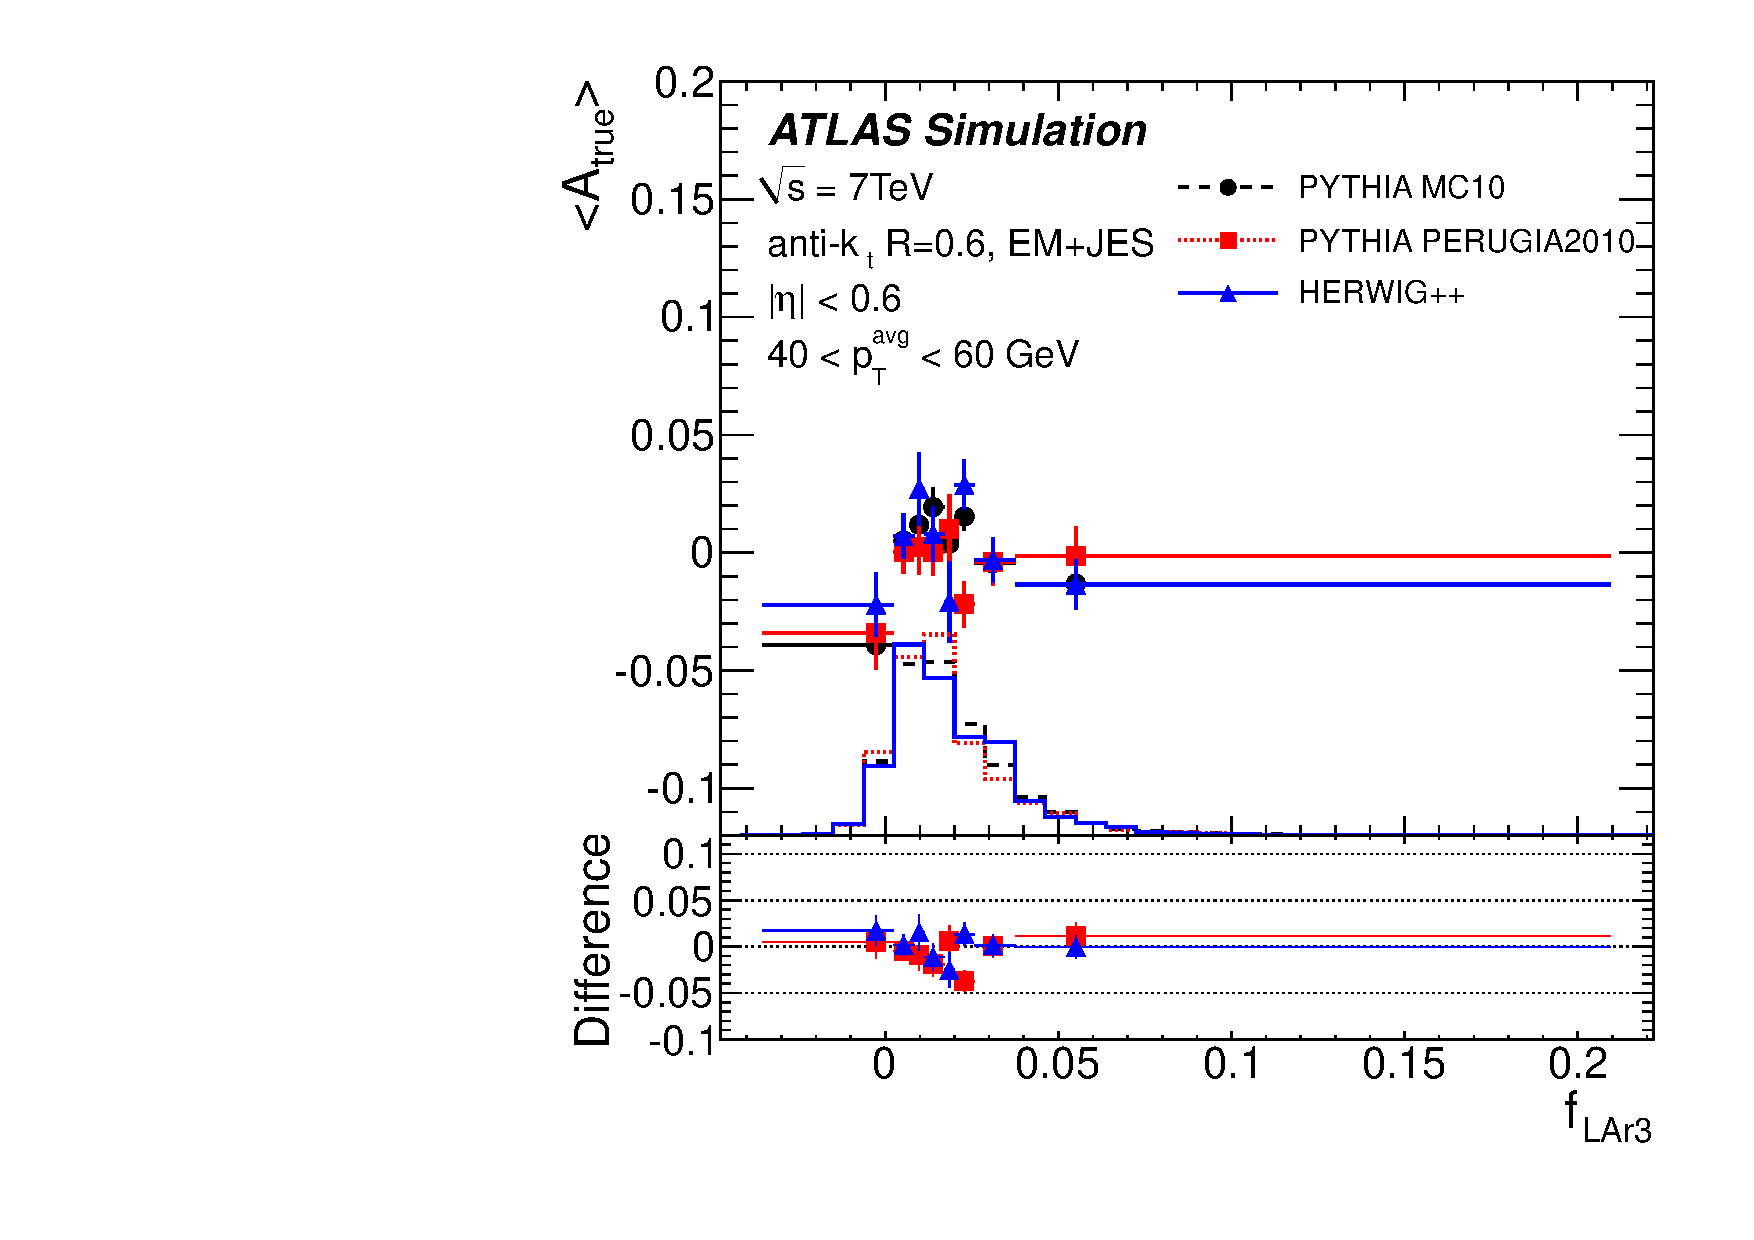
\includegraphics[width=0.4\textwidth]{figures/fig_48b.pdf}\\
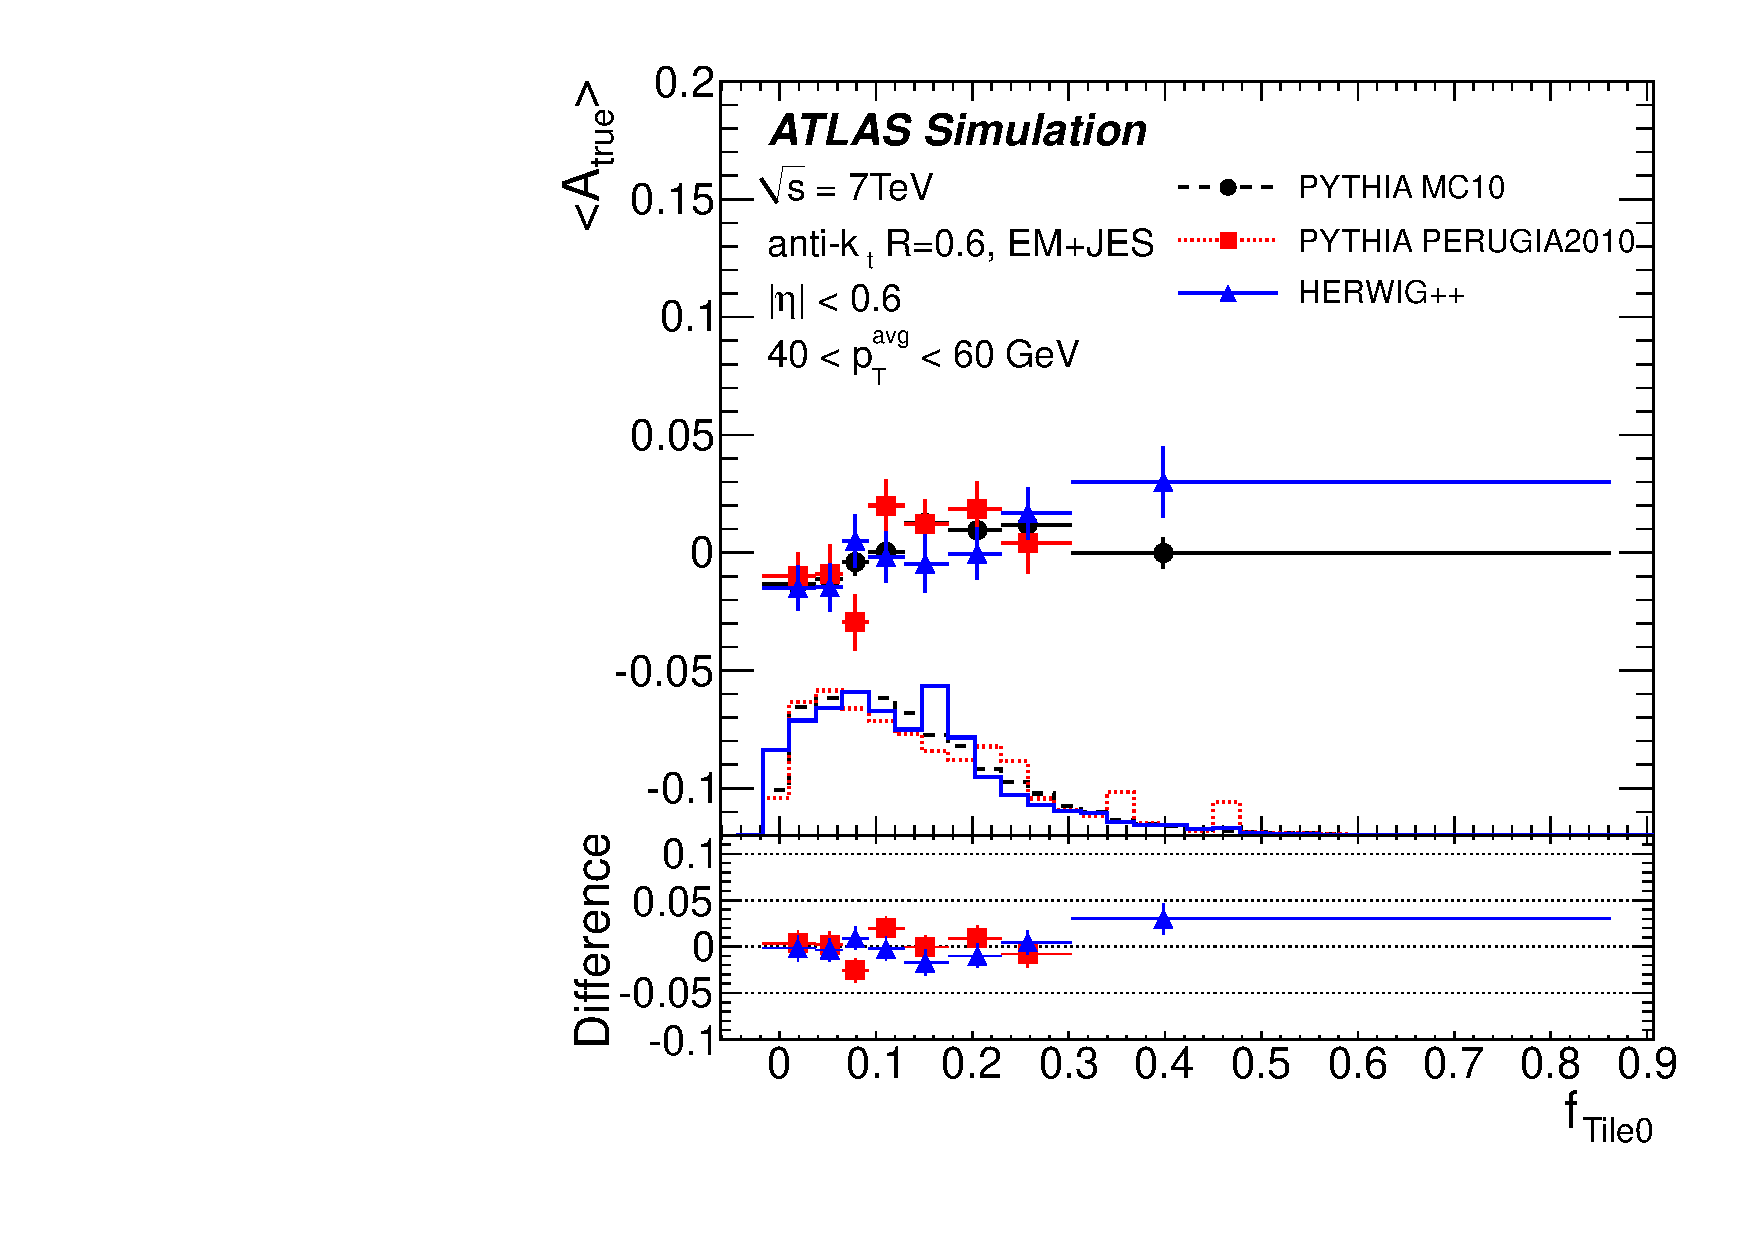
\includegraphics[width=0.4\textwidth]{figures/fig_48c.pdf}
\hspace{1.cm}
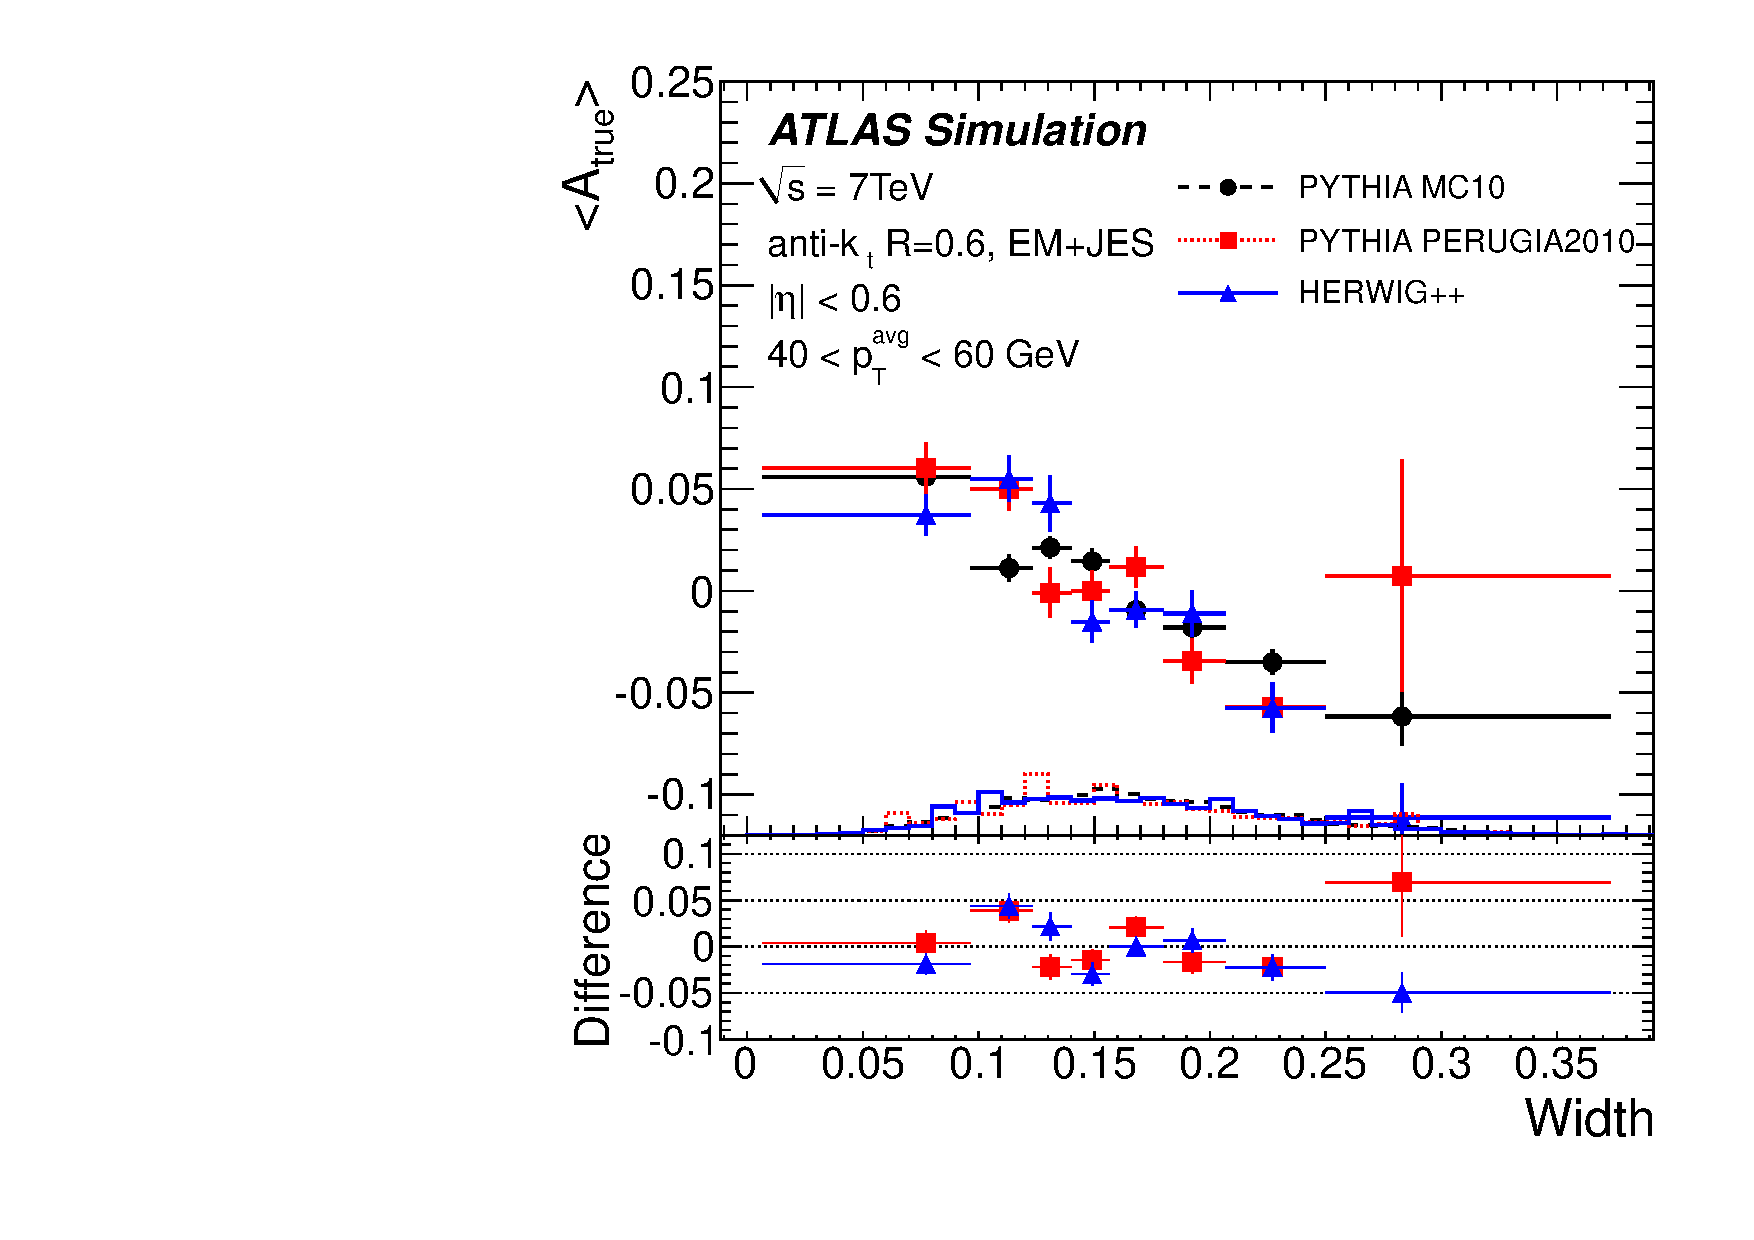
\includegraphics[width=0.4\textwidth]{figures/fig_48d.pdf}
\caption{Asym\'etrie au niveau des jets de particules en fonction des fractions d'\'energie \fpres{}, \fem{}, \ftile{} et de la largeur \width~du jet sonde dans l'\'echantillon simul\'e nominal et dans des \'echantillons avec des mod\'elisation diff\'erentes pour l'hadronisation et les \'ev\'enements sous-jacents (\Perugia2010{} et \herwig++). Les jets ont $40 \le \pt^{\rm avg} < 60$~GeV et $|\eta| < 0,6$. Les distributions des fractions d'\'energie et de la largeur des jets sont montr\'ees, ainsi que les diff\'erences entre l'\'echantillon nominal et les autres.}
\label{fig:AtruthAllSamples}
\end{figure*}

En conclusion, la m\'ethode pr\'esent\'ee dans la section~\ref{sec:DijetBalanceMethod} permet la d\'erivation des coefficients de calibration en fonction des diff\'erentes fractions d'\'energie et de la largeur du jet pour tout l'intervalle en impulsion transverse et en $\eta$ consid\'er\'e. Cette m\'ethode peut par cons\'equent \^etre appliqu\'ee sur les donn\'ees pour valider les corrections calcul\'ees sur la simulation.

\subsubsection{Diff\'erences entre les facteurs correctifs d\'eriv\'ees sur les donn\'ees et sur la simulation}
\label{sec:MCBased_vs_DataBased}

La figure~\ref{fig:DijetMethodDATA} montre les asym\'etrie $A'$ (\'equation~\ref{eq:Aprime} o\`u $A_{\rm true}(x)$ est calcul\'e sur l'\'echantillon \pythia{} nominal) dans les donn\'ees et dans l'\'echantillon \pythia{} nominal en fonction de  $\fpres$, $\fem$, $\ftile$ et de la largeur pour des jets ayant  $80 \le \ptjet < 110$~GeV et $|\eta| < 0,6$. Elles sont compatibles aux incertitudes statistiques pr\`es. Le m\^eme accord est observ\'e dans les autres r\'egions en \eta~ et en \ptjet.

\begin{figure*}[!htb]
\centering
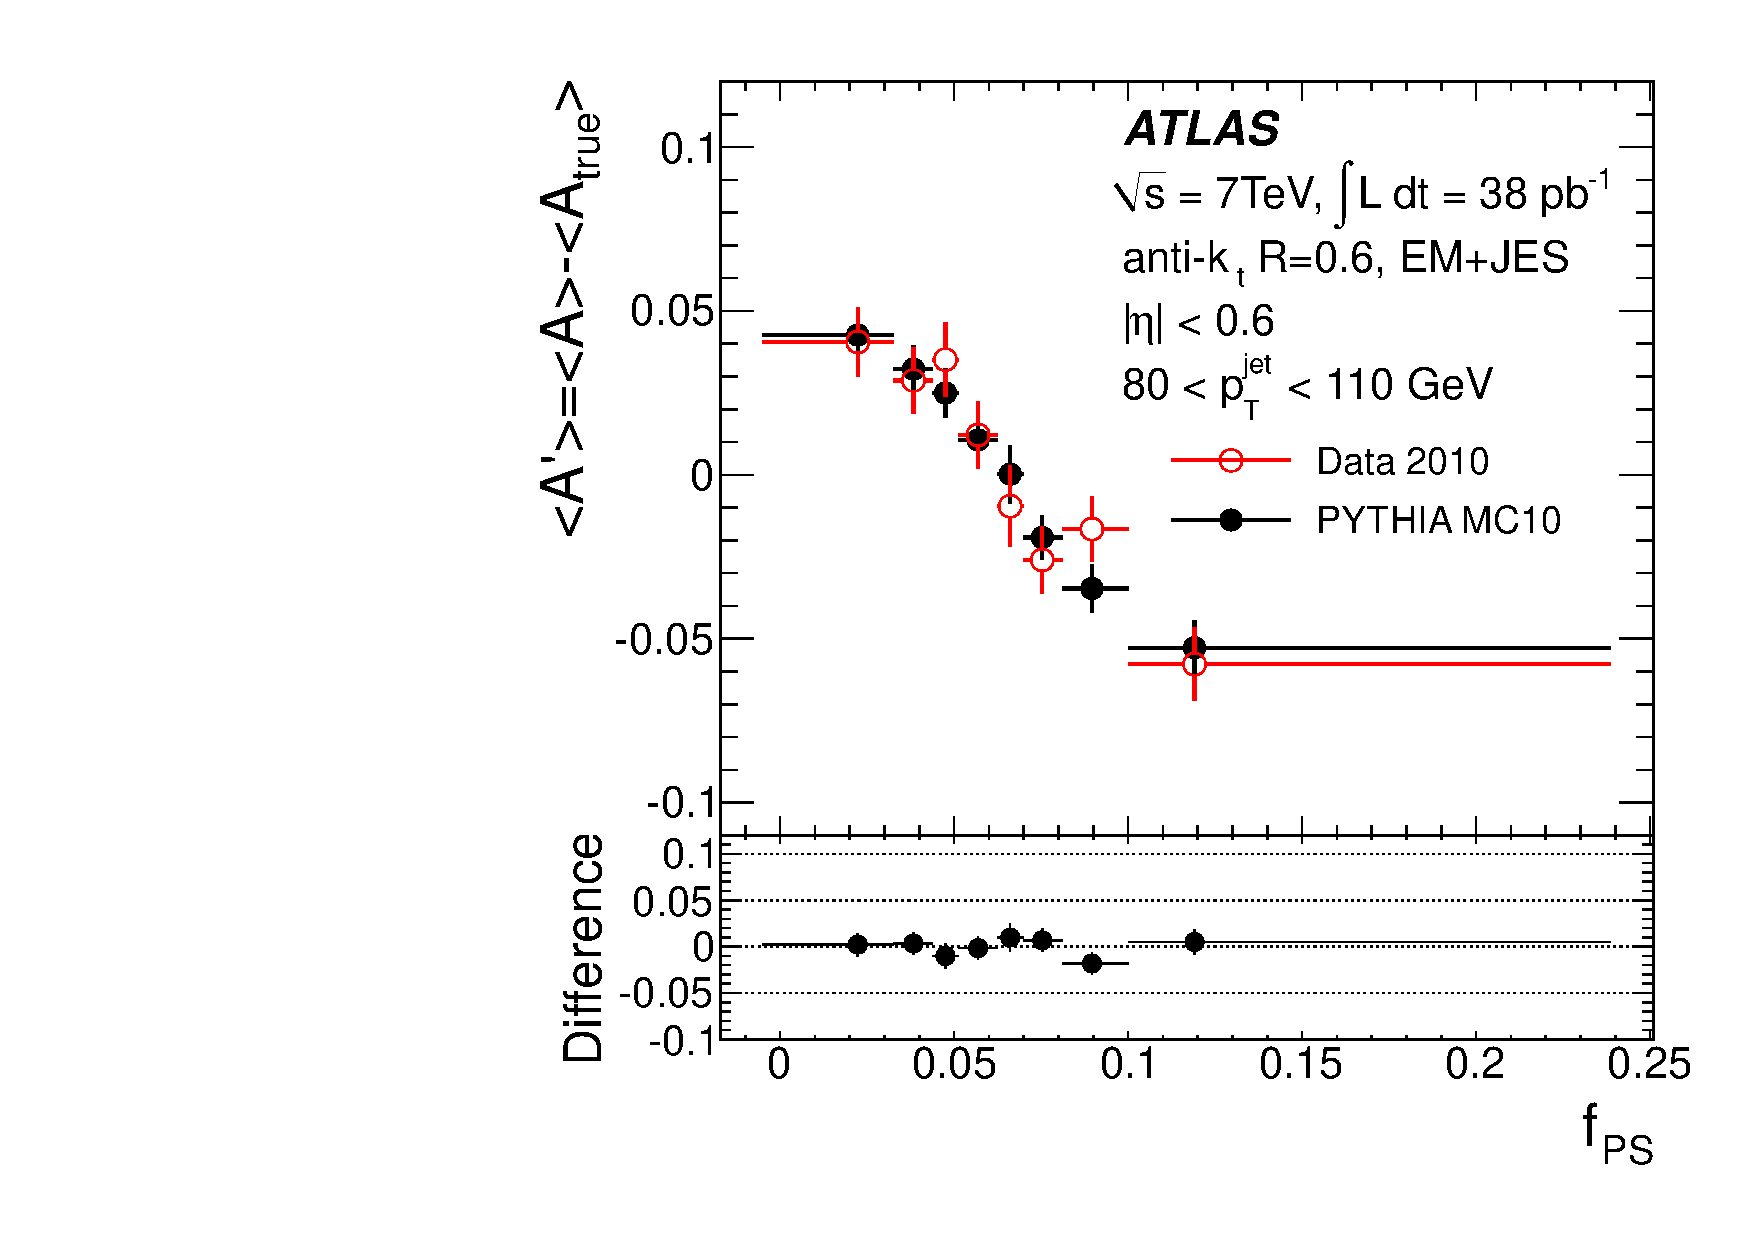
\includegraphics[width=0.4\textwidth]{figures/fig_49a.pdf}
\hspace{1.cm}
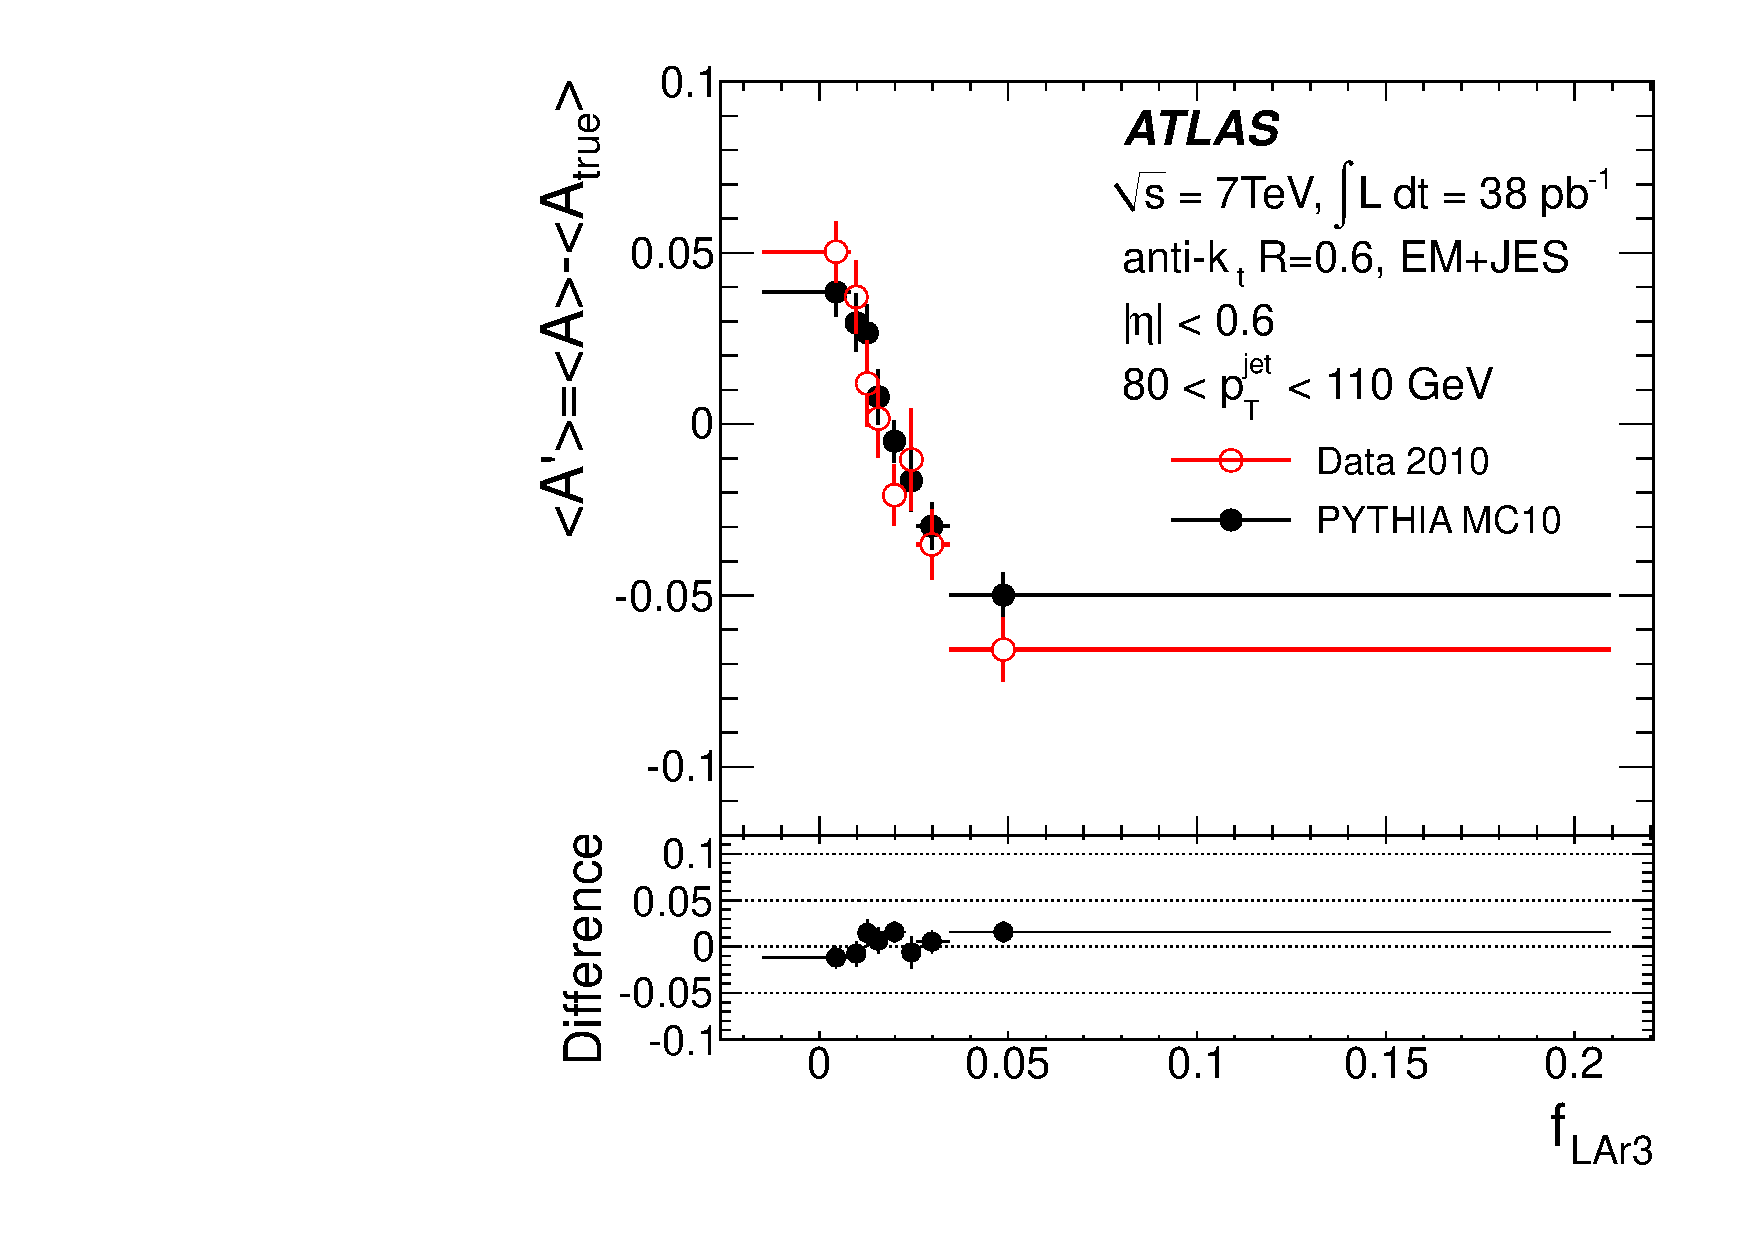
\includegraphics[width=0.4\textwidth]{figures/fig_49b.pdf}\\
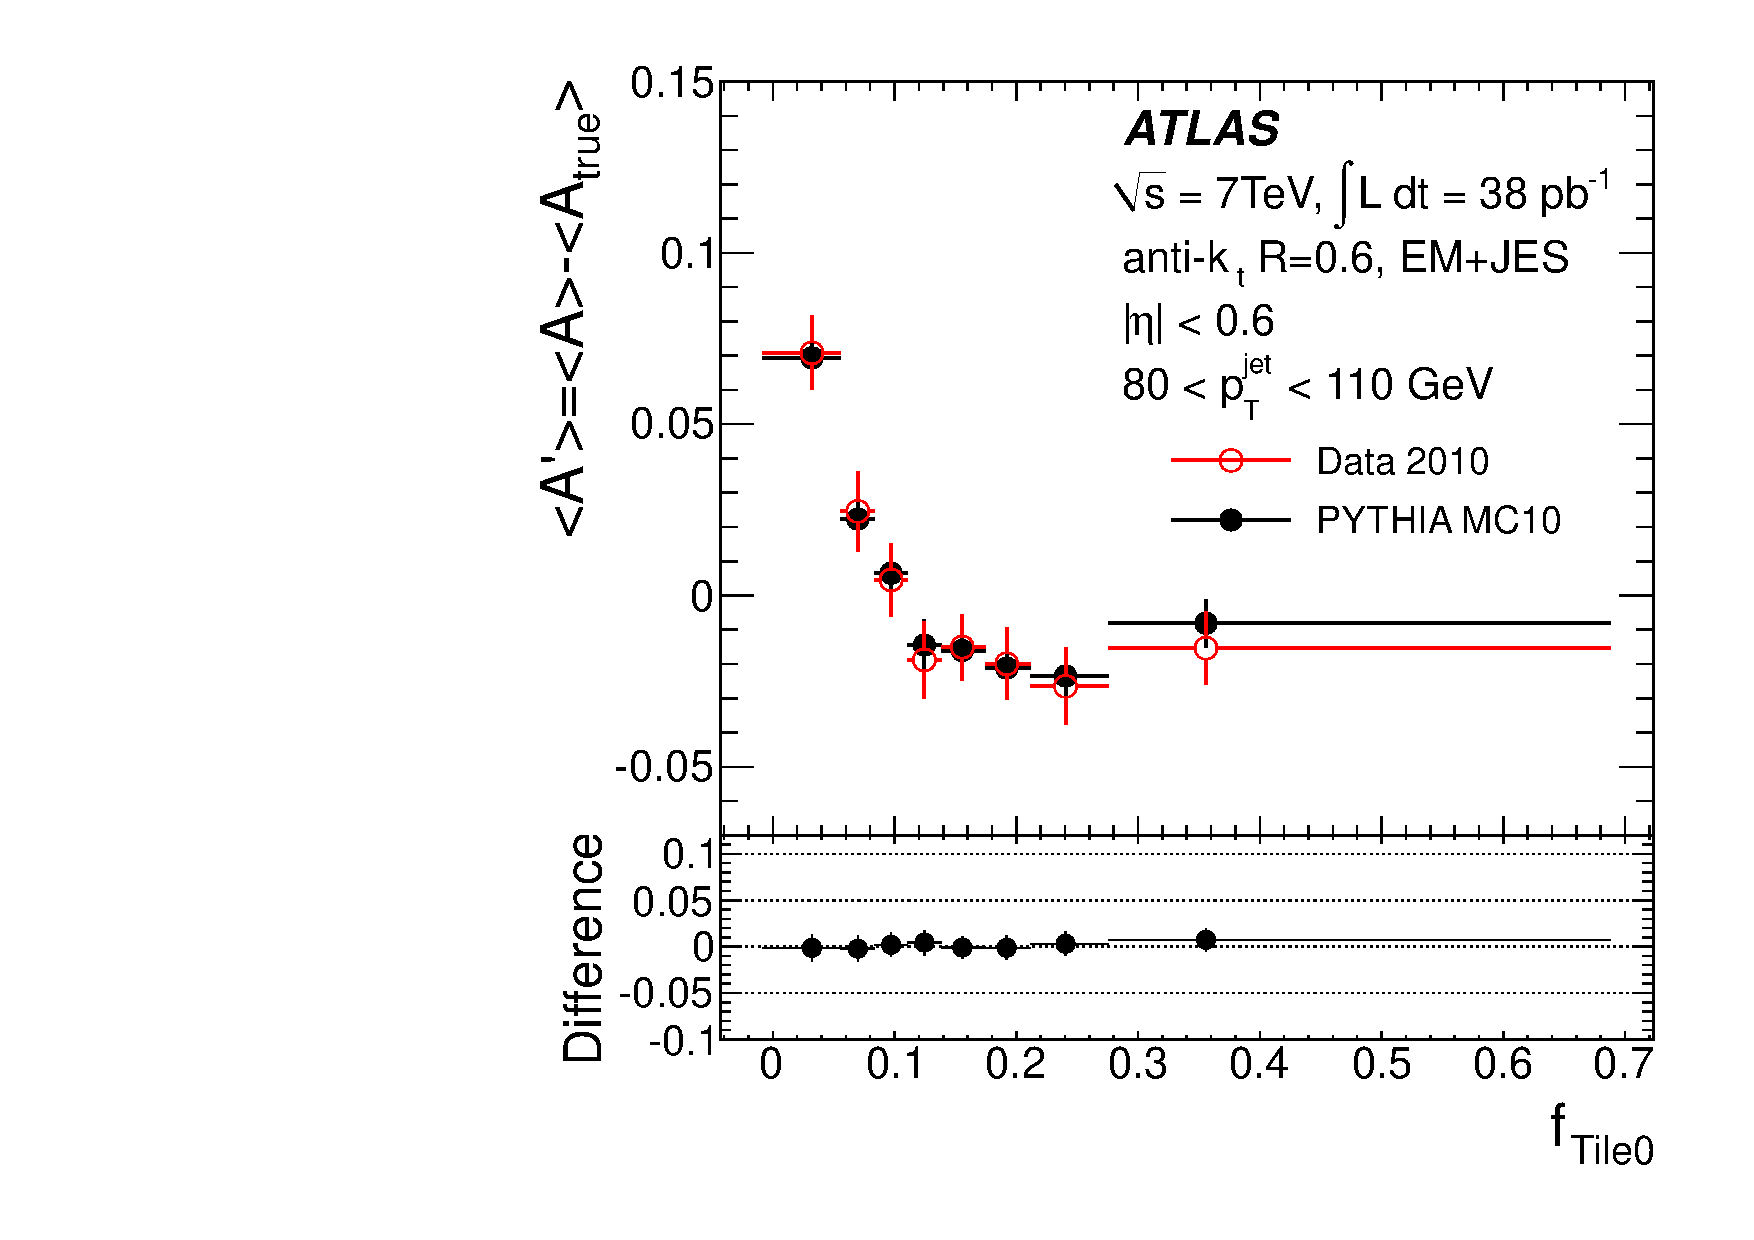
\includegraphics[width=0.4\textwidth]{figures/fig_49c.pdf}
\hspace{1.cm}
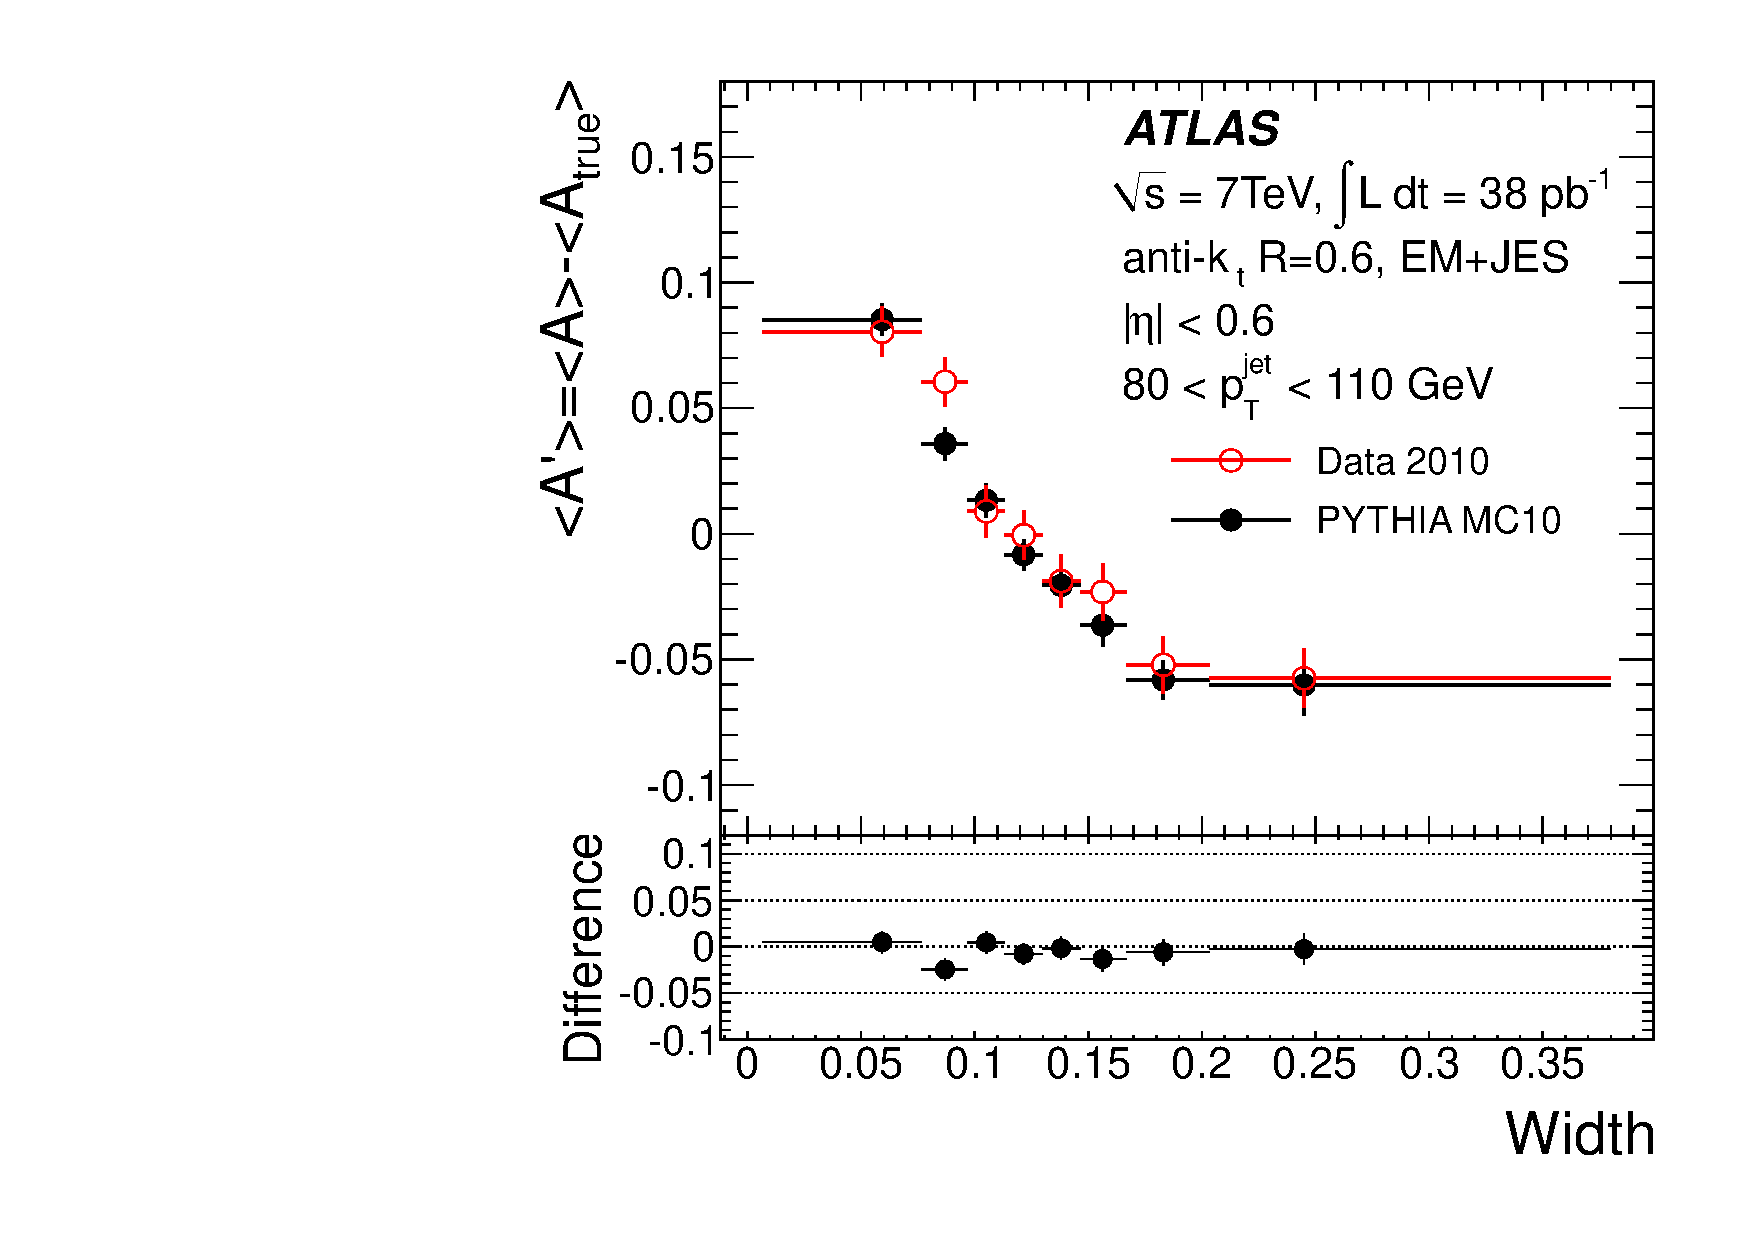
\includegraphics[width=0.4\textwidth]{figures/fig_49d.pdf}
\caption{Diff\'erence entre l'asym\'etrie au niveau des jets calorim\'etriques et l'asym\'etrie au niveau des jets de particules sur les donn\'ees et sur l'\'echantillon simul\'e nominal en fonction de  $\fpres$, $\fem$, $\ftile$ et de la largeur pour des jets ayant  $80 \le \ptjet < 110$~GeV et $|\eta| < 0,6$. Les diff\'erences entre la simulation et les donn\'ees sont montr\'ees en bas de chaque graphique.}
\label{fig:DijetMethodDATA}
\end{figure*}

Les asym\'etries telles que celles montr\'ees sur la figure~\ref{fig:DijetMethodDATA} sont utilis\'ees pour d\'eriver des facteurs correctifs bas\'es sur les donn\'ees. Les diff\'erences de r\'eponse apr\`es application de ces facteurs sur l'échantillon simul\'e nominal mesure l'incertitude syst\'ematique associ\'ee \`a la calibration \GS. Apr\`es les deux premi\`eres corrections (voir table~\ref{tab:properties}), la r\'eponse diff\`ere de moins de $1\%$. Apr\`es les troisi\`eme et quatri\`eme corrections, les diff\'erences augmentent de $1 \%$ \`a $2 \%$ dans la partie centrale du d\'etecteur. Dans la partie bouchon, les diff\'erences sont de $2 \%$ ($4 \%$) pour $\pt^{\rm truth} > 60$~\GeV{} ($ < 60$~\GeV). Il faut toutefois noter que les incertitudes statistiques sur ces diff\'erences sont grandes, s'\'elevant typiquement \`a la moiti\'e de la diff\'erence.

Des facteurs correctifs sur les donn\'ees ont \'egalement \'et\'e calcul\'es en prenant les asym\'etries $A_{\rm true}$ obtenues sur les \'echantillons simul\'es \Perugia 2010 et \herwigpp. Ces corrections sont, comme pr\'ec\'edemment, appliqu\'ees \`a l'\'echantillon simul\'e nominal. Les r\'eponses obtenues sont compar\'ees \`a celles obtenues en appliquant les corrections d\'eriv\'ees des donn\'ees utilisant $A_{\rm true}$ calcul\'e sur l'\'echantillon simul\'e nominal. Les diff\'erences sont inf\'erieures \`a $0,5 \%$ pour tous les intervalles en impulsion transverse et en $|\eta|$ dans lesquels les incertitudes statistiques sont suffisamment petites pour permettre une comparaison pertinente.

Une vérification supplémentaire a été réalisée en appliquant les facteurs correctifs dérivés à partir de la simulation aux données et à la simulation. Les différences de r\'eponse entre données et simulation reflètent les différences dans les propriétés longitudinales et transversales utilisées dans la calibration \GS. La figure~\ref{fig:jetprop_vs_pT} montre la valeur moyenne de $\fpres$, $\fem$, $\ftile$ et de la largeur en fonction de \ptjet~dans la partie centrale du détecteur pour les données et les différents échantillons simulés considérés dans cette étude. Les différences pour $\ftile$ et $\fpres$ entre les données et l'échantillon simulé nominal n'excèdent pas $5 \%$ dans tout l'intervalle en impulsion transverse. Pour $\fem$, les différences n'excèdent pas $5 \%$ non plus sauf pour $20 \le \ptjet < 30$~GeV ou un désaccord de $7.5 \%$ est observé. Un désaccord plus important est observé pour la largeur des jets. Les jets sont plus large de $5 \%$ ($10 \%$) dans les données que dans la simulation à $200$~GeV~($600$~GeV) et plus étroits pour $\pt < 30$~GeV. 
\enlargethispage{0.3cm}
L'écart-type des distributions de \fem~et \fpres~montre également des différences inférieures à $5 \%$ entre données et simulation sur tout l'intervalle en \ptjet. Pour $\ftile$ and \width, des désaccords de $10 \%$ sont observés pour quelques intervalles en impulsion transverse. Des résultats similaires sont trouvés dans les autres régions en $|\eta|$, sauf pour \etaRange{2,1}{2,8}, où l'accord pour la variable \width~est légèrement moins bon.

La figure~\ref{fig:jetprop_vs_pT} montre que les échantillons simulés nominal et \Perugia2010 s'accordent à quelques pourcents. L'accord de l'échantillon \herwig~avec les données est aussi bon que pour les autres échantillons pour $\fem$ et $\ftile$, sauf pour $20 \le \ptjet < 30$~GeV. Pour $\fpres$ et la largeur des jets, des désaccords de $5$ à $10 \%$ sont observés entre \herwigpp~et les autres échantillons pour $\ptjet < 60$~\GeV. Pour $\ptjet > 160$~\GeV, \herwigpp~décrit la largeur des jets mieux que les autres échantillons.

\begin{figure*}[ht!]
\centering
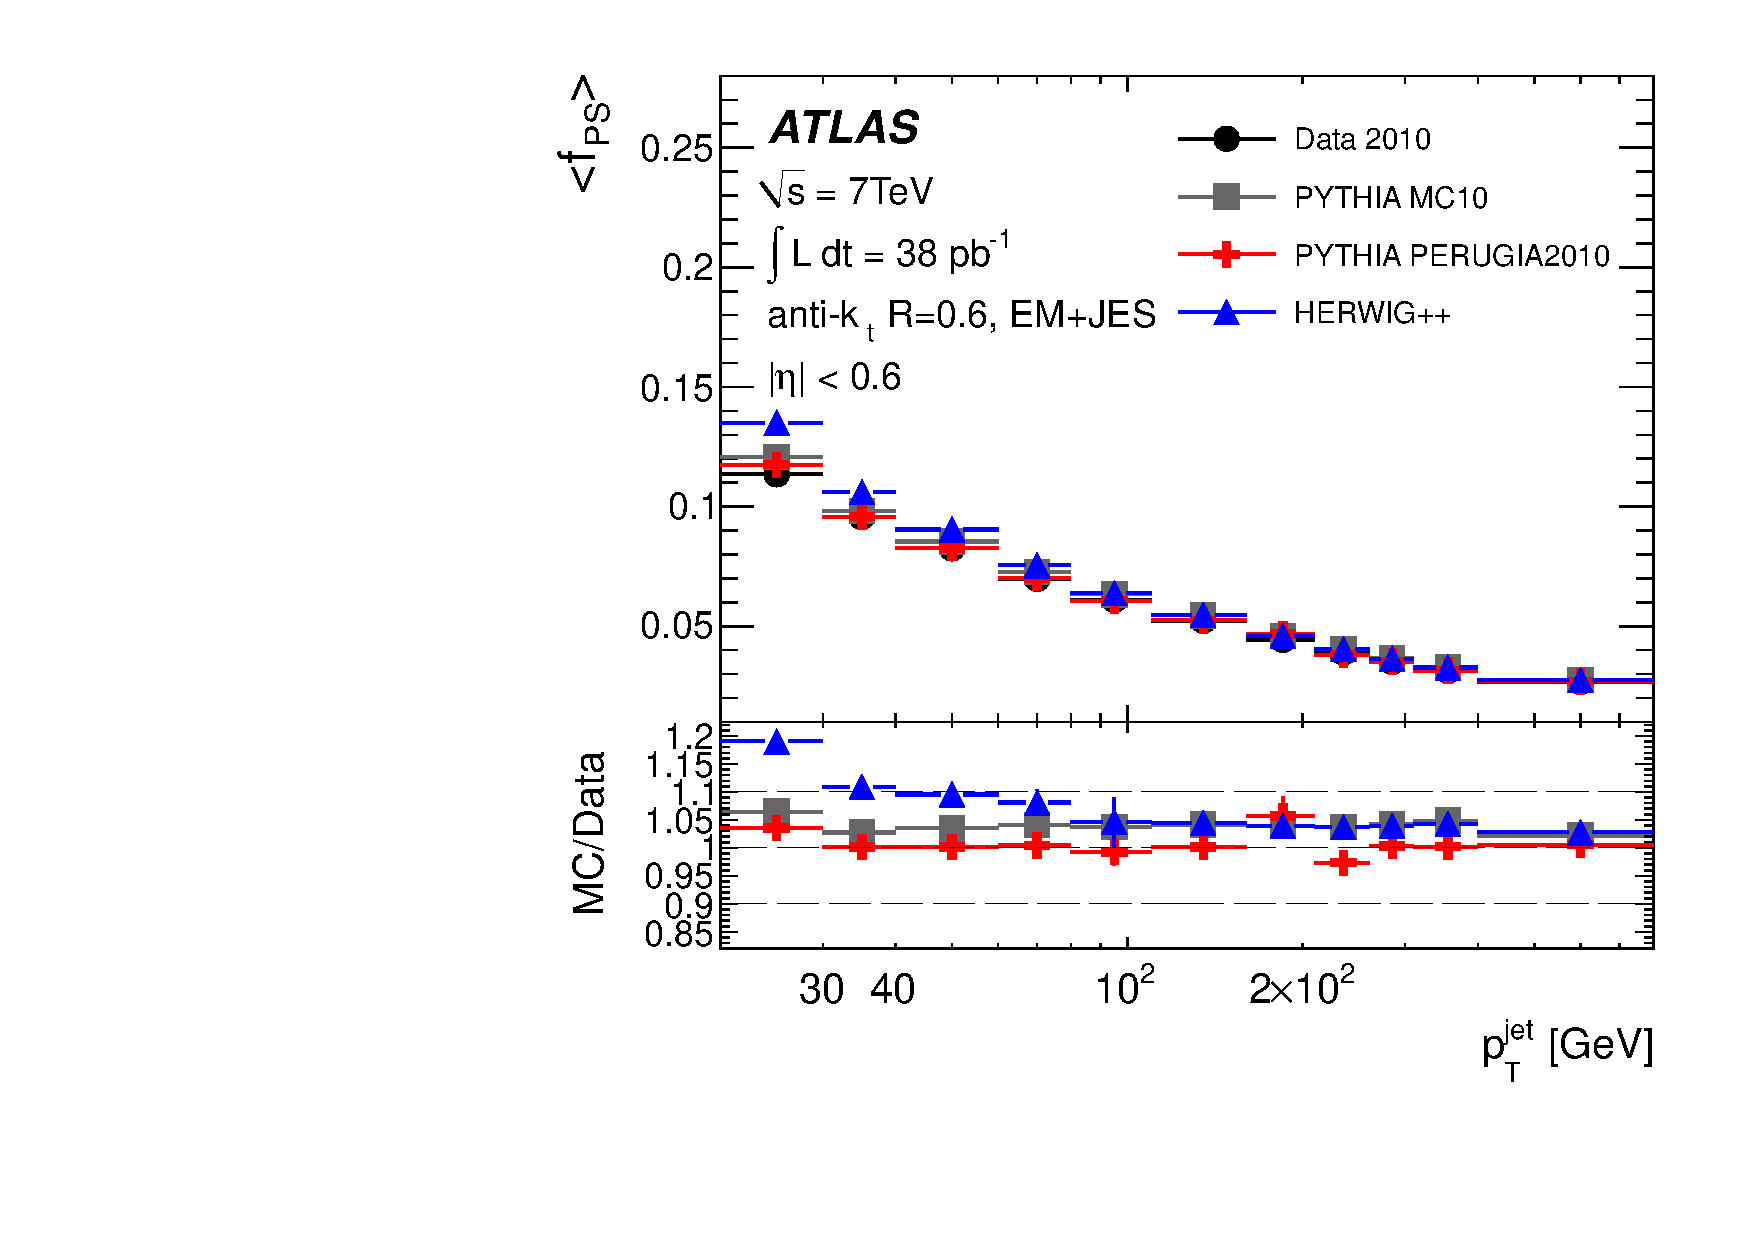
\includegraphics[width=0.4\textwidth]{figures/fig_50a.pdf}
\hspace{1.cm}
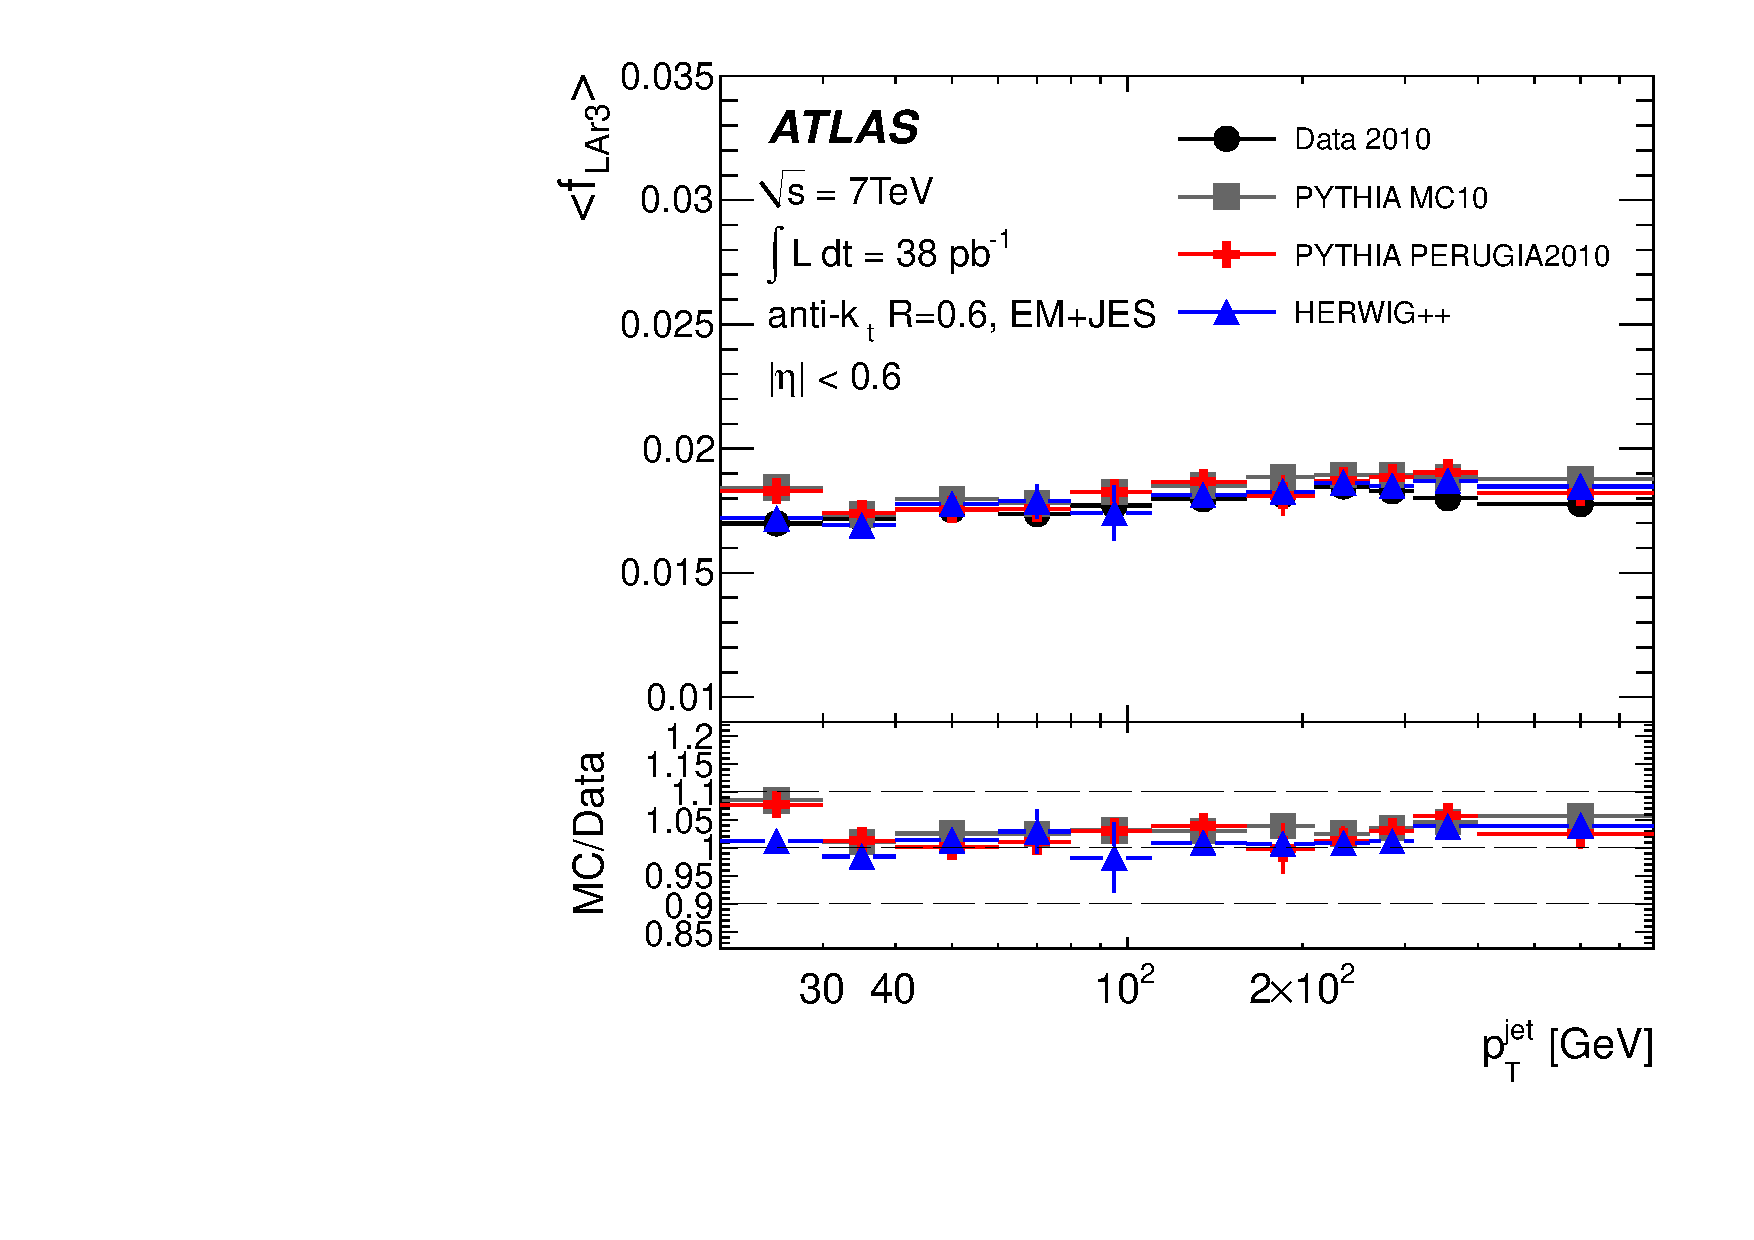
\includegraphics[width=0.4\textwidth]{figures/fig_50b.pdf}\\
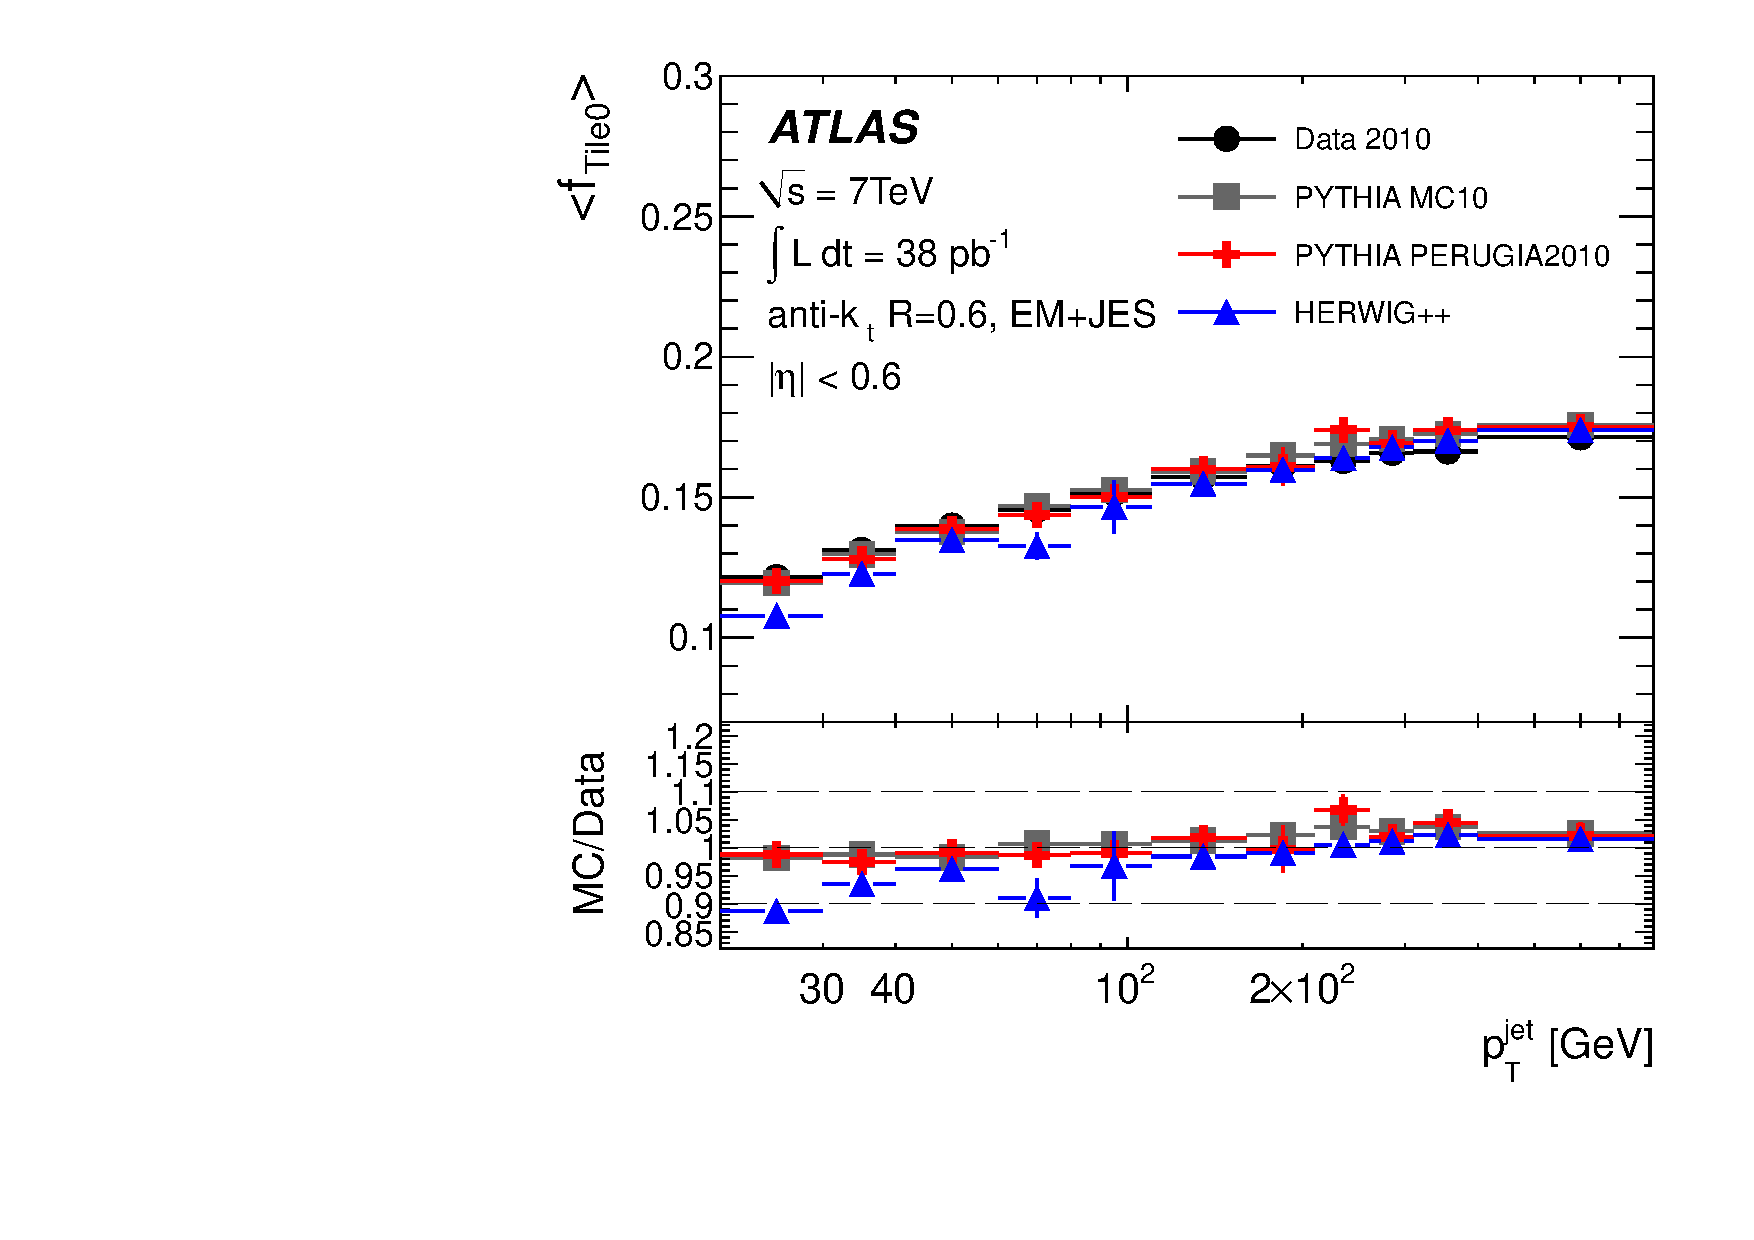
\includegraphics[width=0.4\textwidth]{figures/fig_50d.pdf}
\hspace{1.cm}
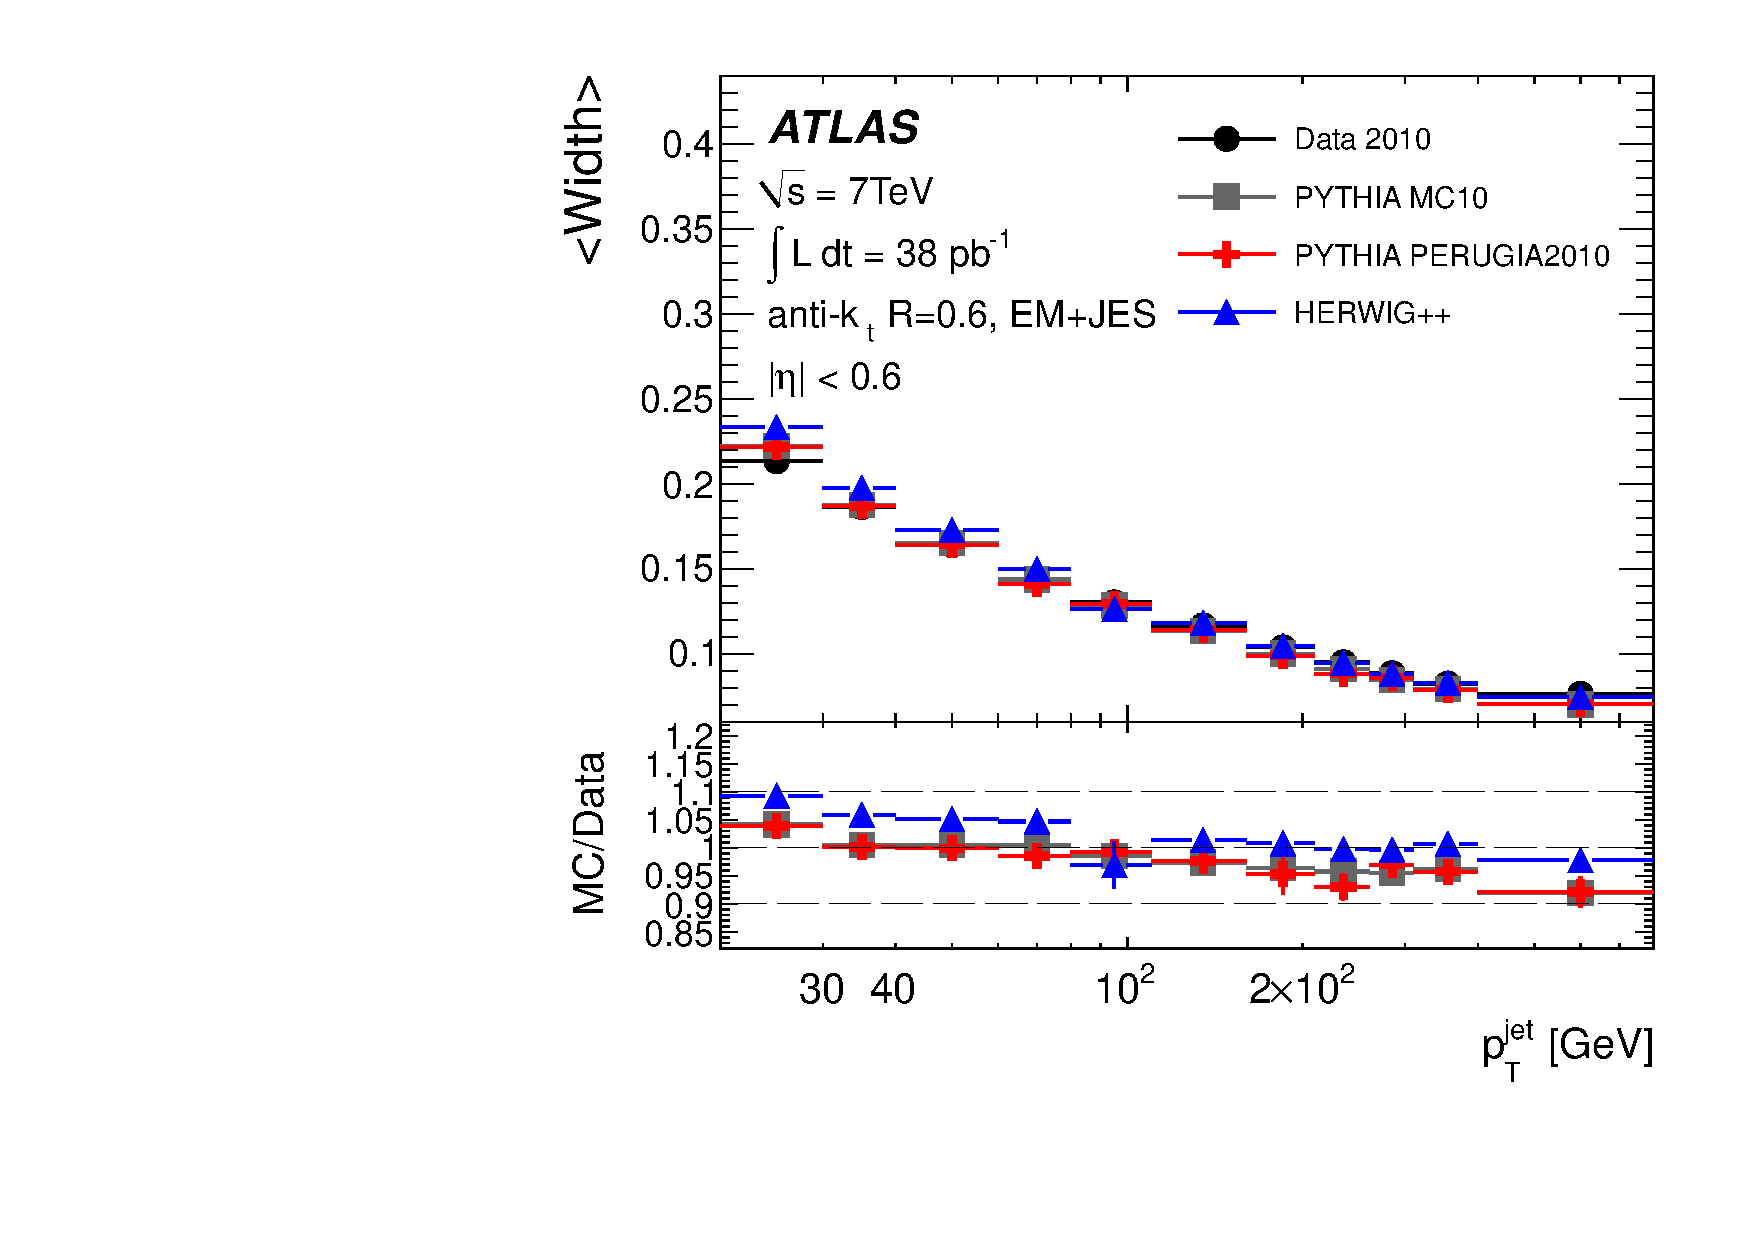
\includegraphics[width=0.4\textwidth]{figures/fig_50c.pdf}
\caption{Valeur moyenne des fractions d'\'energie $\fpres$,  $\fem$, $\ftile$ et de la largeur $\width$~en fonction de \pt~pour $|\eta| < 0,6$ dans les donn\'ees et les simulations. Le rapport entre les simulations et les donn\'ees sont montr\'es en bas de chaque graphique.}
\label{fig:jetprop_vs_pT}
\end{figure*}

L'incertitude systématique peut être estimée quantitativement en évaluant les différences de facteurs correctifs $E_{\GS}^{\rm jet}/E_{\EMJES}^{\rm jet}$ entre les données et la simulation. 
Les facteurs correctifs en fonction de \ptjet~dans la région centrale et de $\eta$ pour $80 \le \ptjet < 110$~GeV dans les données et l'échantillon simulé nominal après \GSL~et \GS~sont montrés sur la figure~\ref{fig:EcalEem}. 
Le rapport entre données et simulation est montré en bas de chaque figure. 
%La figure~\ref{fig:EcalEem} montre la même quantité mais en fonction de $\eta$ pour $80 \le \ptjet < 110$~GeV. 
L'écart à l'unité dans le rapport représente l'incertitude systématique associée à la calibration \GSL~ou \GS. En général, il est inférieur à 1\% pour $20 \le \ptjet < 800$~GeV et \etaRange{0}{2,8}.


\begin{figure*}[ht!]
\centering
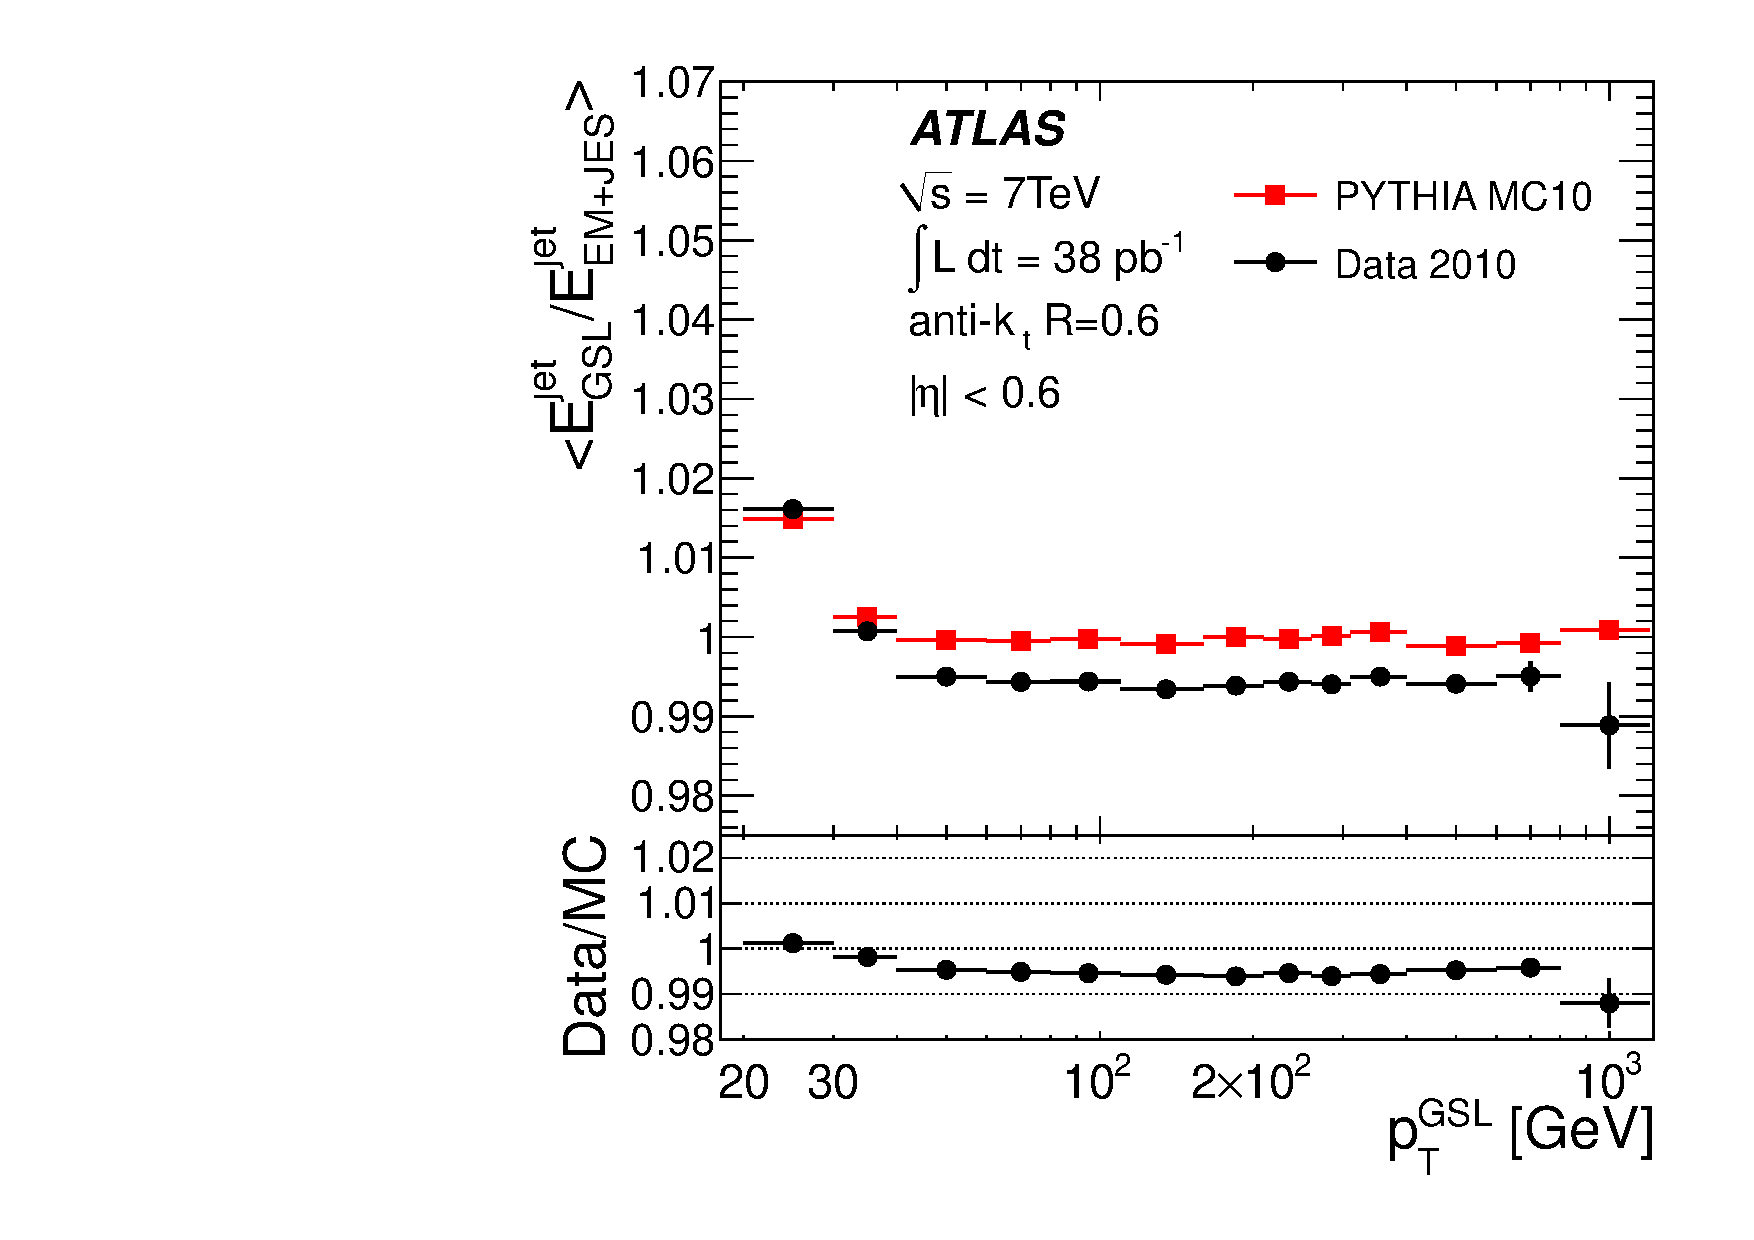
\includegraphics[width=0.4\textwidth]{figures/fig_51a.pdf}
\hspace{1.cm}
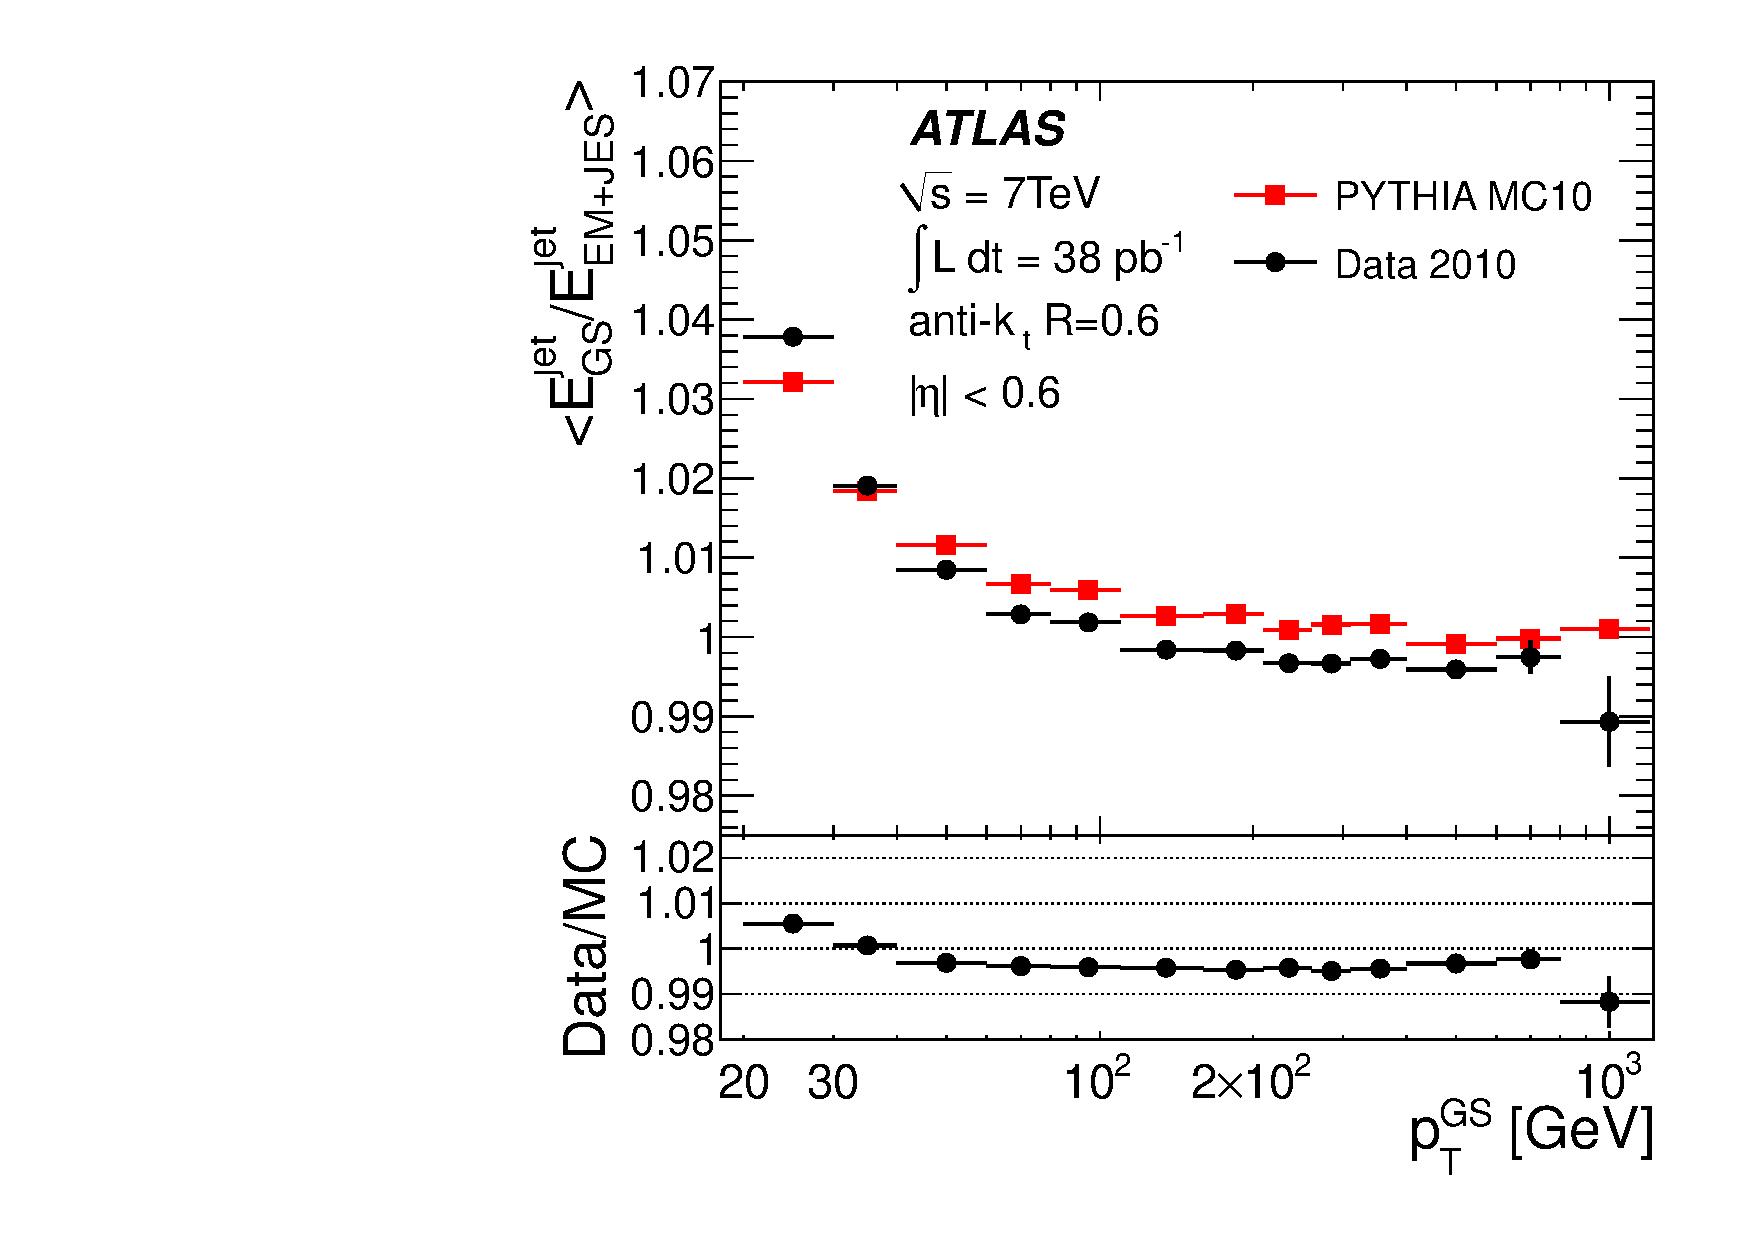
\includegraphics[width=0.4\textwidth]{figures/fig_51b.pdf}\\
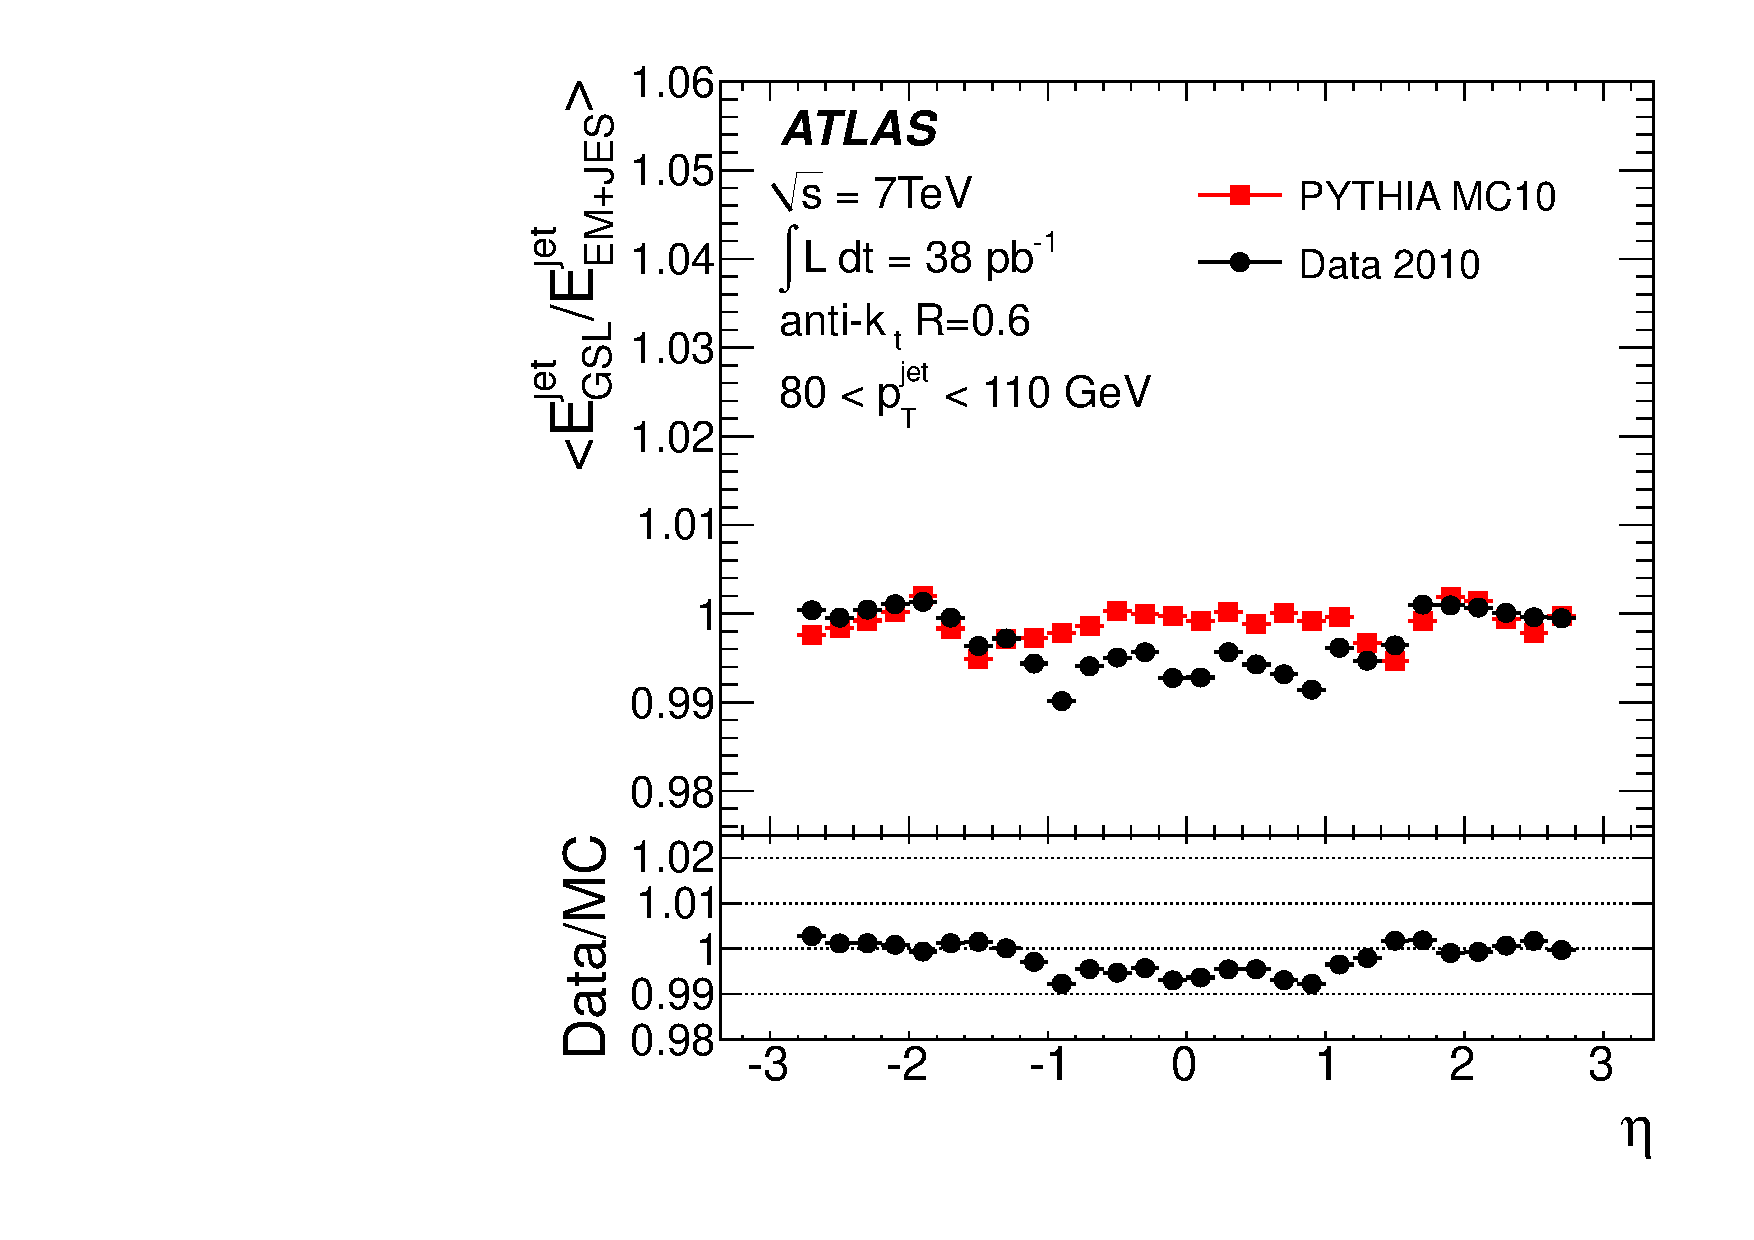
\includegraphics[width=0.4\textwidth]{figures/fig_51c.pdf}
\hspace{1.cm}
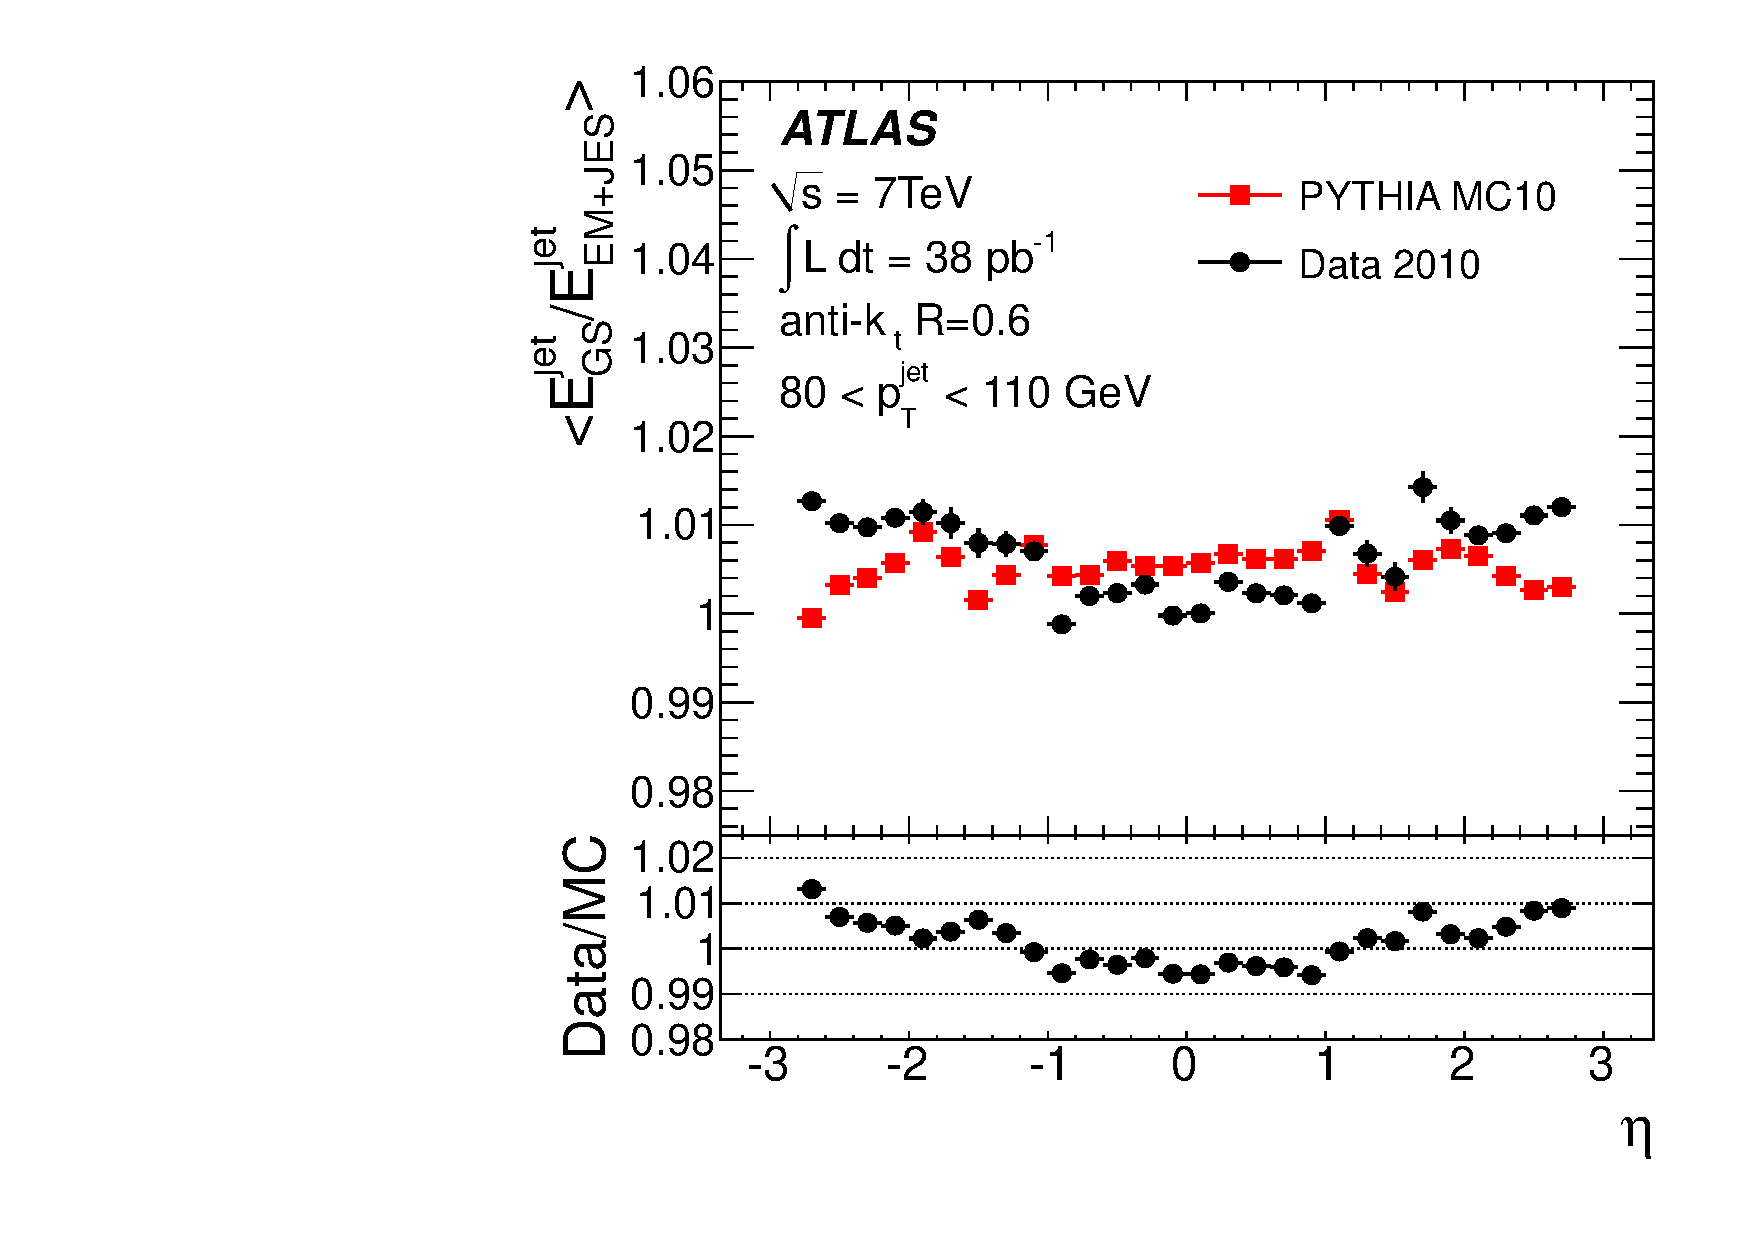
\includegraphics[width=0.4\textwidth]{figures/fig_51d.pdf}
\caption{Moyenne du facteur correctif pour les calibrations \GSL{} (\`a gauche) et \GS{} (\`a droite) en fonction de \ptjet{} (en haut) dans la partie centrale du calorim\`etre et de \eta{} pour $80 \le \ptjet < 100$~GeV (en bas) dans les donn\'ees et la simulation. Le rapport entre les donn\'ees et la simulation est montr\'e en bas de chaque graphique.}
\label{fig:EcalEem}
\end{figure*}

%This uncertainty is added in quadrature to the \EMJES{} uncertainty.
%The results for all the \ptjet{} and $\eta$ ranges are the following:

%For $20 \le \ptjet < 30$~\GeV{} and \etaRange{0}{2.1}, the data to Monte Carlo ratio varies from $0.5 \%$ to $0.7 \%$ depending on the $|\eta|$ region. For $\ptjet > 30$~\GeV{} and \etaRange{0}{2.1}, the uncertainty is lower than $0.5 \%$. For \etaRange{2.1}{2.8}, the the data to Monte Carlo ratio varies from $0.4 \%$ to $1 \%$ depending on the \ptjet{} bin. For a given \ptjet, the uncertainty is higher for \etaRange{2.1}{2.8} than for \etaRange{0}{2.1}, because of the poorer description of the jet width. For \etaRange{2.1}{2.8} the \GSL{} scheme shows slightly larger difference than the \GS{} scheme.In general, the uncertainty on the data to Monte Carlo ratio is lower than $1 \%$ for $20 \le \ptjet < 800$~\GeV{} and \etaRange{0}{2.8}.

L'incertitude ayant pour origine la mauvaise description des propriétés longitudinales et transversales dans la simulation et les différences entre les facteurs correctifs dérivés à partir des données et ceux dérivés sur la simulation présentées dans la section~\ref{sec:MCBased_vs_DataBased} ne sont pas indépendantes. La réponse en énergie après la calibration \GS~(ou \GSL) dans chaque intervalle en \ptjet~et \eta, qui dépend des distributions des propriétés et des facteurs correctifs eux-m\^eme, est proche de la réponse après calibration \EMJES. Un changement dans la distribution d'une propriété se propage par conséquent au facteur correctif en fonction de cette propriété de telle sorte que la réponse reste inchangée dans l'échantillon utilisé pour dériver la correction. Les différences observées dans la section~\ref{sec:MCBased_vs_DataBased} sont donc en partie dues à des différences dans les distributions des propriétés et pas seulement à des diff\'erences dans les facteurs correctifs.

\subsection{Sensibilité de la calibration GS~aux effets d'empilement}

Un propriété très intéressante de la calibration \GS~qui a été observée au cours de ces études est sa relative indépendance vis-à-vis des effets d'empilement attendus dans les données de 2010. 
Les distributions des propriétés et les facteurs correctifs varient en effet peu lorsque des événements supplémentaires sont ajoutés à l'interaction principale. 
Les corrections dérivées en l'absence d'empilement sont donc applicables aux échantillons avec empilement, la dégradation dans l'échelle en énergie étant minime. 
\enlargethispage{0.5cm}
L'estimation quantitative des effets d'empilement est obtenue en applicant la calibration \GS~dérivée dans l'échantillon simulé nominal (sans empilement) à des échantillons avec empilement. La réponse résultante est comparée à la réponse après application de la calibration \EMJES, dans laquelle l'énergie additionnelle liée à l'empilement est soustraite. La réponse après les différentes corrections de la calibration \GS~change de moins de $1\%$ ($2\%$) pour $\pt > 30$~GeV ($\pt < 30$~GeV). Ces variations sont inférieures à l'incertitude sur l'échelle en énergie sans empilement, et ceci quelque soit l'impulsion transverse.

%Les conditions d'empilement étant très différentes à la fin du run 1 et au début du run 2 qu'au début du run 1, il serait nécessaire de reproduire cette étude pour savoir si les conclusions tirées ci-dessus sont toujours valables. 

\section{Conclusion}

Les \'etudes pr\'esent\'ees dans ce chapitre montrent que la calibration \GS{} permet une am\'elioration substantielle de la calibration des jets par rapport \`a la calibration \EMJES. 
Ces am\'eliorations portent principalement sur la r\'esolution en \'energie et la d\'ependance de l'\'echelle en \'energie avec la saveur. De plus, l'incertitude syst\'ematique associ\'ee \`a la calibration \GS{} est inf\'erieure \`a 1\% pour \etaRange{0}{2,8} et $20 \le \ptjet < 800$~\GeV. Les sources responsables de cette incertitude sont largement d\'ecorr\'el\'ees de celles responsables de l'incertitude sur la calibration \EMJES. L'incertitude sur la calibration \GS{} peut par cons\'equent \^etre ajout\'ee en quadrature \`a celle sur la calibration \EMJES~(figure~\ref{fig:fig_22a_JES2010UncertaintyCentral}). La d\'egradation de l'incertitude sur l'\'echelle en \'energie apr\`es calibration \GS{} est donc minime. 

Ces r\'esultats ont conduit la collaboration \ATLAS~\`a poursuivre le d\'eveloppement et l'\'etude des performances de la calibration~\GS{} apr\`es publication de~\cite{Aad:2011he}. L'effet de cette calibration (dans une version l\'eg\`erement modifi\'ee par rapport \`a celle pr\'esent\'ee dans ce chapitre) a notamment \'et\'e \'etudi\'e dans la recherche du boson BEH se d\'esint\'egrant en une paire $b\bar{b}$~\cite{Aad:1541965}. Il a \'et\'e montr\'e que \GS{} permet une am\'elioration de la r\'esolution sur la masse invariante de la paire $b\bar{b}$ d'environ 8\% par rapport \`a la calibration~\EMJES. Cette calibration a par cons\'equent \'et\'e utilis\'ee~pour la recherche $H\rightarrow b\bar{b}$ avec les donn\'ees \`a $\sqrt{s}=8~$TeV~\cite{Aad:2014xzb}. 

La calibration \GS{} fait aujourd'hui partie de la calibration officielle des jets dans \ATLAS{} o\`u elle est utilis\'ee conjointement avec la calibration \LCW. L'application s\'equentielle de ces deux calibrations permet de b\'en\'eficier des avantages propres \`a chacune d'elle : la calibration des gerbes calorim\'etriques gr\^ace \`a \LCW{} et les faibles r\'esolution et incertitude syst\'ematique gr\^ace \`a \GS.















